%TODO:  
%  (from data) say how many times destroy and reconstruct, average how many rooms were destroyed.
%	 Add dollar graphs

%  Add experimental results using different neighbourhoods
%  Add concept of LNS, symmetry
%     Say today solver such as cplex, gurobi can do symmetry detection, however it is more effective by leveraging on knowledge on problem structure
%  Add SMAC - how smac works and other parameter tuning software
%  Add different way of neighourhood...say pros and cons



%%%%

%%%%


\chapter{Scaling to Large Problems}
\label{cha:lns}

\section{Introduction}

In Chapter~\ref{cha:milp} we showed that combining HVAC control with occupancy scheduling can lead to substantial improvements in energy efficiency. Our MIP-based joint model achieves a significant energy reduction when compared to the existing state-of-the-art approaches \citep{goyal2013occupancy,kwak2013tesla,majumdar2012energy,chai2014minimizing}.
%those heuristic-based energy-aware scheduling approaches that assume a black-box model for HVAC control \citep{kwak2013tesla,majumdar2012energy,chai2014minimizing}. 
Given the highly-constrained nature of occupancy scheduling with HVAC control, solving the integrated problem as a MIP seems to be a reasonable choice. MIP easily manages the interaction between occupancy scheduling and the impact it has on HVAC energy consumption. The problem with the MIP-based approach, however, is that it does not scale. It only allows us to solve small problem instances in reasonable time. 

In Chapter \ref{cha:milp} Section \ref{sec:mip:experiments}, the largest instances we tackle consist of 4 rooms and 50 meetings over 5 days. When the problem size increases to a larger number of rooms and number of meetings, for example 20 rooms and 200 meetings, MIP's convergence becomes very slow and sometimes fails to occur after a day. This is a common problem in a MIP model involving symmetry. Symmetry exists in a MIP model when integer variables can be permuted without changing the structure of the problem \citep{margot2010symmetry}. This property greatly affects the branch-and-bound process in MIP. 
Technically, symmetries can be removed effectively by taking advantage of a problem structure. This includes grouping the variables with identical properties into one group or imposing an ordering to the variables by lexicographic constraints.
% or leveraging on the structure of the problem and introducing symmetry breaking constraints (eg. impose an ordering to the variables by introducing lexicograpic constraints). 
This is a technique regarded as \textsl{symmetry breaking}\footnote{Most of the existing optimisation solvers \citep{gurobi, cplex2009v12} also support problem-independent symmetry breaking technique, which solely depend on the MIP model. They provide a configurable parameter that activates automatic detection and removal of symmetries in MIP. However, it is stated at \cite{gurobisym} that changing the value of this parameter rarely produces a significant benefit.}. In our model, a large number of 
\vspace*{-2px}
\begin{enumerate}
	\item meetings with similar properties (eg. number of attendees, meeting time windows, room capacity, equipments required etc.),    \label{sym1} 
	\item rooms with similar temperature and temperature fluctuation rates, and  \label{sym2}
	\item scheduling periods with low diurnal temperature variation.  \label{sym3}
\end{enumerate}
\noindent form symmetries or near-symmetries that lead to slow convergence. 
The first type of symmetries \eqref{sym1} can be tackled using the grouping approach. These are common in scheduling problems, where many meetings (a.k.a jobs) have identical properties. To overcome this, we can reformulate the model so that these meetings with similar properties are grouped, thus exploiting the symmetries in \eqref{sym1}. Unfortunately, for symmetry types \eqref{sym2} and \eqref{sym3}, as the rooms temperatures fluctuate according to occupancy, two rooms with similar properties may have different temperatures depending on the scheduled meeting allocations, hence resulting in an asymmetrical state. Therefore it is impossible to group them into one room type. This leads to multiple symmetric optima with very small differences that renders branch-and-bound in MIP ineffective. The latter is in fact a ''near-symmetric`` problem that cannot be solved effectively via symmetry breaking, and has been an open problem in MIP for a long time \citep{ostrowski2010symmetry}. Fortunately, given the detailed understanding of the HVAC control and occupancy scheduling problem, it is possible to exploit the model structure to overcome these issues. 

In this chapter, we adopt a hybrid solution that combines MIP with large neighbourhood search (LNS) to solve our joint control and scheduling problem. The advantage is twofold. This strategy copes with symmetries and near-symmetries in a MIP-based system based on our understanding on the problem structure. It also scales our joint model to handle problem sizes that, for example, companies and universities may face when scheduling meetings and lectures. A commercial office or an university building typically consists of multiple floors with a lot of rooms. In order to consolidate energy-efficient schedules, a meeting appointment or an university timetabling application needs handle large number of activities across these rooms. For example, about 300 meetings have to be scheduled every weekday across 35 study rooms in the main library of University Southern California \citep{kwak2013tesla}. These bookings are handled by a centralized online room reservation system. Meanwhile, night and weekend classes were consolidated from 21 buildings to 5 buildings in \cite{portland:2012} to reduce energy consumption. Thus, it is crucial for our joint model to handle these large instances and produce near-optimal control and scheduling solutions, given sets of activity requests with different constrainedness and sets of buildings with varying thermal response.

We extend our work in Chapter \ref{cha:milp} and develop an approach that scales to larger problems by combining MIP with LNS. LNS is used to destroy part of the schedule and MIP is used to repair the schedule so as to minimise energy consumption. This approach is far more effective than solving the complete problem as a MIP problem. Our results show that solutions from the LNS-based approach are up to 36\% better than the MIP-based approach when both are given 15 minutes. 

The remainder of this chapter is organized as follows. 
Section \ref{sec:lns} describes the LNS model. We discuss in turn our LNS algorithm, the formulation of initial solution, the destroy and repair steps, and finally the LNS parameter tuning. 
Section \ref{sec:lns_mip} highlights the MIP model formulation for the LNS initialization stage and the MIP model reduction to remove symmetries and speed up our joint model. 
We present our experimental results in Section \ref{sec:results} and review the related work in Section \ref{sec:related_work}.
Finally, we conclude with key observations and opportunities for further work in Section \ref{sec:lns:conclusion}.

%---------------------------------
\section{Large Neighborhood Search}\label{sec:lns}

LNS is a local search metaheuristic, which was originally proposed by \cite{shaw1998using}. In LNS, an initial solution is improved iteratively by alternating between a destroy and a repair step. The main idea behind LNS is that a large neighbourhood allows the heuristic to easily navigate through the solution space even when the problem is highly-constrained. This is opposed to a small neighbourhood, which may make escaping a local minimum much harder. Algorithm \ref{alg:lns} outlines our LNS approach. 

\begin{algorithm}[ht!]
\small
%\SetAlgoLined
\SetKwFunction{Return}{return}
\SetKwInput{Input}{Input}
\SetKwInput{Output}{Output}
\SetKwInput{Initialize}{Initialization}
\SetKwInput{Algorithm}{Destroy \& Repair}
\SetKwIF{If}{ElseIf}{Else}{if}{then}{else if}{else}{endif}
 \Indm
 \Input{Meeting requests $M$, Rooms $L$, time steps $K$}
 \Output{Master Schedule $S$, Energy Consumption $J$ }
 \Initialize{}
 \Indp{$S \gets \emph{GenInitialMeetingSchedule}(M, L, K)$\\
$ J \gets \emph{GenHVACControl}(S)$
 }\\
 \Indm
 \Algorithm{}
 \Indp
 \While{not LnsTimeUp()}
 {
	$L' \gets \emph{SelectNeighborhood}\left(L\right)$ \\
	$\emph{DestroyNeighborhood}\left(S, M(L'), L' \right)$ \\
	$\langle S', J' \rangle \gets \emph{RepairNeighborhood}\left(S, M(L'), L' \right)$\\
	\If{$J' < J$}	
	{
		$J \gets J' $\\
		$\emph{UpdateSchedule}\left(S', S \right)$
	}
 }
 \Return $S$
 \caption{LNS approach}
 \label{alg:lns}
\end{algorithm}

\subsection{Initialization Phase}\label{sec:lns_init}

Our LNS approach starts with an initial feasible solution, which is generated using a greedy heuristic. First, this heuristic finds a feasible meeting schedule by minimising the number of rooms in which meetings are located. As we saw in Chapter \ref{cha:milp}, this is a commonly used heuristic in energy-aware meeting scheduling. Second, it determines the HVAC control settings of supply air temperature and supply air flow rate to minimise energy consumption given the fixed schedule. This two-stage approach allows us to come up with an initial solution in reasonable time.


\subsection{Destroy \& Repair}\label{sec:lns_dr}

Next, we run multiple iterations of destroy and repair steps to re-build and re-optimise the selected neighbourhoods. An important decision in the destroy step is determining the amount of destruction. If too little is destroyed the effect of a large neighbourhood is lost, but if too much is destroyed then the approach turns into repeated global re-optimisation. As for the repair step, an important decision is whether the repair should be optimal or not. An optimal repair will typically be slower than a heuristic, but may potentially lead to high quality solutions in a few iterations. As a result, a neighbourhood destroy and repair strategy is essential in achieving good performance overall.

Our LNS approach considers a room-based neighbourhood that contains a subset of the rooms or zones. In particular, we destroy the schedule in two to four randomly selected rooms. This forms a subproblem that can be solved effectively using MIP. When destroying meetings in more than four zones, MIP performance can degrade very quickly and even solving the linear programming relaxation can become quite time consuming. The repair consists in solving an energy aware meeting scheduling problem that is much smaller than the original problem. We do, however, limit MIP runtime to avoid excessive search during a repair step, and to avoid any convergence issues of the MIP problem. Setting a limit on runtime means that we do not necessarily solve the subproblem to optimality, but given that MIP solvers are anytime algorithms, we do improve solution quality in many of the LNS iterations. If we find an improved solution, then the new schedule and control settings are accepted. Otherwise, we maintain the solution that was just destroyed. Given that the LNS starts with a feasible solution and does not accept infeasible solutions, the solution remains feasible throughout the execution of the algorithm.

We should note that we have experimented with a variety of neighbourhoods. These include: destroying all meetings in randomly selected time steps, a combination of destroying all meetings in randomly selected rooms and time steps, and simply destroying a set of randomly selected meetings. Our observation was that none of these neighbourhoods performed as well as destroying all meetings in a number of randomly selected rooms. Destroying selected rooms means that meetings could be rescheduled at any time during the day. This allows the model to optimise supply air flow rate and supply air temperature over all the time steps. Destroying selected time steps means that meetings may switch rooms, but may need to be scheduled to the same time step due to time window restrictions. This limits the optimisation of supply air flow rate and supply air temperature due to the HVAC control constraints on neighboring time steps.

%There is a correlation between the time windows selected for HVAC control! Hence infeasible solution may happen... etc.


\subsection{LNS Parameter Tuning}\label{sec:lns_param}

In order to fine-tune the LNS heuristic we apply automatic parameter tuning, which is a useful step in producing better results on average.
The parameters that govern the behavior of the LNS heuristic are parameters determining the probability of destroying a number (2, 3, or 4) of rooms and the MIP runtime limit for the repair step. The probabilities on the number of rooms to destroy are defined as a 3-tuple with values ranging between [0,1] and the MIP runtime limit is a parameter with values ranging between 1 and 10 seconds. 

While it is possible to reason about certain parameters and their impact on overall performance, these parameters can take infinitely many values. Even though we consider only 4 parameters, it is impossible to try all possible configurations because of their continuous domains. Note, even with discretized domains with reasonable level of granularity it remains impractical to try out all configurations. As a result, we use the automated algorithm-configuration method called Sequential Model-based Algorithm Configuration (SMAC) \citep{hutter2011sequential} to optimise these parameters.

SMAC can be used to train parameters in order to minimise solution runtime, or to optimise solution quality. In our case, we fix the runtime and minimise energy consumption. We generate problem instances with different degrees of constrainedness and train the parameters to achieve the average best quality for all input scenarios.

Given a list of training instances and corresponding feature vectors, SMAC learns a joint model that predicts the solution quality for combinations of parameter configurations and instance features. This information is useful in selecting promising configurations in large configuration spaces. For each training instance we computed up to 17 features, including: 
\iffalse
(1) number of constraints, (2) number of variables, (3) number of non-zero coefficients, (4) number of meetings, (5) number of meeting types, (6) scheduling flexibility, (7) average duration of meetings, (8) number of meeting slots per day, (9) total number of meeting slots, (10)-(14) number of rooms in up to 5 building types, and (15)-(17) minimum, maximum, and average difference between outdoor temperature and temperature comfort bounds.
\fi
\begin{itemize}
\item number of constraints, 
\item number of variables, 
\item number of non-zero coefficients, 
\item number of meetings, 
\item number of meeting types, 
\item number of possible starting time slots (scheduling flexibility), 
\item average duration of meetings, 
\item number of meeting slots per day, 
\item total number of meeting slots, 
\item number of rooms in our 5 building types (defined in Chapter \ref{cha:milp}, Table \ref{tab:rc_wall_win}), and 
\item minimum, maximum, and average difference between outdoor temperature and temperature comfort bounds.
\end{itemize}
These features reflect problem characteristics and are used by SMAC to estimate performance across instances and generate a set of new configurations.

Given a list of promising parameter configurations, SMAC compares them to the current incumbent configuration until a time limit is reached. Each time a promising configuration is compared to the incumbent configuration, SMAC runs several problem instances until it decides that the promising configuration is empirically worse or at least as good as the incumbent configuration. In the latter case the incumbent is updated. In the end, the configuration selected by SMAC is generalized to all problem instances in the training set. For more details about SMAC, we refer readers to \cite{hutter2011sequential}.

%When the problem only involves a small number of rooms then IP can be quite effective. We exploit this observation be\varphi\varphi\varphi\varphi\varphi

% Talk about using probability to decide whether to destroy 2, 3, or 4 rooms, instead of an arbitrary input.



\section{MIP Model}\label{sec:lns_mip}

In this section, we present our MIP formulations that are used with LNS. We first describe the MIP model that generates an initial feasible solution.  Then we present a reduced model that removes symmetries in meeting requests and simplifies the thermal dynamics model. This reduced model is adopted in the initialization phase, as well as the destroy and repair steps. At the end, we recap the equations that is used in each phase.

% Rewrite this... not only apply to initial phase of the lNS, also destroy and repair
%In this section, we present our MIP formulations for the\textcolor[rgb]{1,0,0}{ initial phase of the LNS}. We first describe the model that generates an initial feasible solution. Then we present a reduced model that removes symmetries in meeting requests and simplifies the thermal dynamics model. At the end, we recap the joint model that is used in the destroy and repair steps.

\subsection{Initialization Phase}

%we present our MIP formulations for the\textcolor[rgb]{1,0,0}{ initial phase of the LNS}.
%Our goal is to generate an initial feasible solution as quickly as possible. This can be achieved by first generating a valid schedule, i.e. a schedule where all meetings are assigned and none of the scheduling constraints presented in Section \ref{sec:mip:scheduling} are violated. Instead of randomly assigning meetings to any room (while obeying all constraints), we adopt a heuristic by scheduling these meetings in minimum number of rooms at each day across the scheduling period. Thus, the objective function is defined as minimising the room used per day. Let $d = \left\{1,...,D\right\}$ be a set of day across the scheduling period with $D$ days. Let $K_d = k_{(d-1) \times N},...,k_{d \times N-1}$ be an ordered set of time steps belongs to day $d \in D$, $N$ is a constant denoting the total time slot per day (in our case, N=48) and $K_d \subseteq K$. The objective function is defined as 

Our goal is to generate an initial feasible solution as quickly as possible. This can be achieved by first generating a valid schedule, i.e. a schedule where all meetings are assigned and none of the scheduling constraints presented in Section \ref{sec:mip:scheduling} are violated. Instead of randomly assigning meetings to any room (while obeying all constraints), we adopt a heuristic that schedules these meetings in the minimum number of rooms each day across the scheduling period. Let D be the set of days across the scheduling period. Moreover, let $\func{day-of}: K \rightarrow D$ be the function giving the day in which time step $k$ starts, i.e. $\func{day-of}(k) = ((k-1) \div N) +1$, where $N$ is the number of time steps per day and $\div$ is the integer division. The objective function is defined as


%BAV_y_LD_0_1 + BAV_y_LD_0_2 + BAV_y_LD_0_3 + BAV_y_LD_0_4
   %+ BAV_y_LD_0_5 + BAV_y_LD_1_0 + BAV_y_LD_1_1 + BAV_y_LD_1_2
   %+ BAV_y_LD_1_3 + BAV_y_LD_1_4 + BAV_y_LD_1_5 + BAV_y_LD_2_0
   %+ BAV_y_LD_2_1 + BAV_y_LD_2_2 + BAV_y_LD_2_3 + BAV_y_LD_2_4
   %+ BAV_y_LD_2_5 + BAV_y_LD_3_0 + BAV_y_LD_3_1 + BAV_y_LD_3_2
   %+ BAV_y_LD_3_3 + BAV_y_LD_3_4 + BAV_y_LD_3_5
\begin{equation} \label{eq:objective_minr}
\mbox{minimise: } \sum_{l \in L, d \in D} y_{l,d}
\end{equation}

\noindent where,
% CSTR_MinRoom_MLK_0_0_210: BDV_x_MLK_0_0_210 - BAV_y_LD_0_4 <= 0
% CSTR_MinRoom_MLK_0_0_211: BDV_x_MLK_0_0_211 - BAV_y_LD_0_4 <= 0
% CSTR_MinRoom_MLK_0_1_210: BDV_x_MLK_0_1_210 - BAV_y_LD_1_4 <= 0
% CSTR_MinRoom_MLK_0_1_211: BDV_x_MLK_0_1_211 - BAV_y_LD_1_4 <= 0
% CSTR_MinRoom_MLK_1_1_162: BDV_x_MLK_1_1_162 - BAV_y_LD_1_3 <= 0
% CSTR_MinRoom_MLK_1_1_163: BDV_x_MLK_1_1_163 - BAV_y_LD_1_3 <= 0
\begin{equation} \label{eq:ms_minroomalloc} 
x_{m,l,k} \leq y_{l,d} \hspace{10pt} \forall m \in M, l \in L_m, k \in K_m, d = \func{day-of}(k)
\end{equation}

%\begin{equation} \label{eq:ms_minroomalloc} 
%x_{m,l,k} \leq y_{l,d} \hspace{10pt} \forall m \in M, l \in L_m, k \in K_m, d \in D_m
%\end{equation}

\noindent Recall that the variable $x_{m,l,k}$ equals to 1 if meeting $m$ is scheduled to start at time step $k$ in zone $l$ and equals to 0 otherwise. The binary variables $y_{l,d}$ determine if zone $l$ is being occupied in day $d$. Constraints \eqref{eq:ms_minroomalloc} set the value of $y_{l,d}$ to 1 when at least one meeting starts at zone $l$ at day $d$.

%\noindent Recall that the variable $x_{m,l,k}$ equals to 1 if meeting $m$ is scheduled to start at time step $k$ in zone $l$ and equals to 0 otherwise. The binary variables $y_{l,d}$ determine if zone $l$ is being occupied in day $d$. Constraints \eqref{eq:ms_minroomalloc} set the value of $y_{l,d}$ to 1 when at least one meeting starts at zone $l$ at day $d$. We let $D_m$ be the set of days that meeting $m$ can start, that is $D_m = \left\{D' \subseteq D | \forall k \in K_m, d \in D', k \in K_d\right\}$. 

With this, the initial schedule is generated by adding objective function \eqref{eq:objective_minr} and Constraints \eqref{eq:ms_minroomalloc} with Constraints \eqref{eq:ms_every}-\eqref{eq:ms_meeting} in Section \ref{sec:mip:scheduling}. Compared to randomly assigning meetings to any room, this approach packs as many meetings as possible in the same room at different day across the scheduling period. While scheduling meetings back-to-back does not necessary lead to an optimal solution, we recognize that it is a heuristic that generates a reasonably good initial solution for HVAC control. In the best case scenario, all meetings are assigned to the most energy-efficient room(s), and a good solution can be generated in the initial stage. To diversify the search space and avoid the worst case scenario where all meetings are assigned to a room that consumes a lot of energy, we bound these constraints in a daily basis so that meetings can be packed in different rooms at different days of the scheduling horizon. 

This initial schedule is then fed into our occupancy-based HVAC control model in Section \ref{sec:mip:control} to generate an optimal HVAC control setting. In this initialization phase, the first stage consists of an IP model where the decision variables are all integer variables. This model can be solved effectively using the state-of-the-art MIP solvers such as Gurobi \citep{gurobi}. 
Once the room and time allocations for all meetings have been identified, the second stage consists of a MIP model which need only optimise all continuous decision variables $a^{SA}_{l,k}$ and $T^{SA}_{l,k}$, and if standby mode is enabled, the binary variables $w_{l,k}$, for the HVAC control. As such, by decomposing the joint model into two-stages, our model can yield an initial solution quickly. 


\subsection{Model Reduction}

% Say Now we switch MIP formulation reduction, that apply to all MIP model in initial phase and destroy and repair steps...
In this section, we discuss two model reduction approaches that improve the performance of our MIP model. These approaches are applied to the MIP models in the initialization phase, as well as the destroy and repair steps. The resulting reduced model greatly improves the branch-and-bound of the MIP model, without compromising on the accuracy of the model.


\subsubsection{Removing Symmetries in Meetings}

\begin{figure}[b]
	\centering
		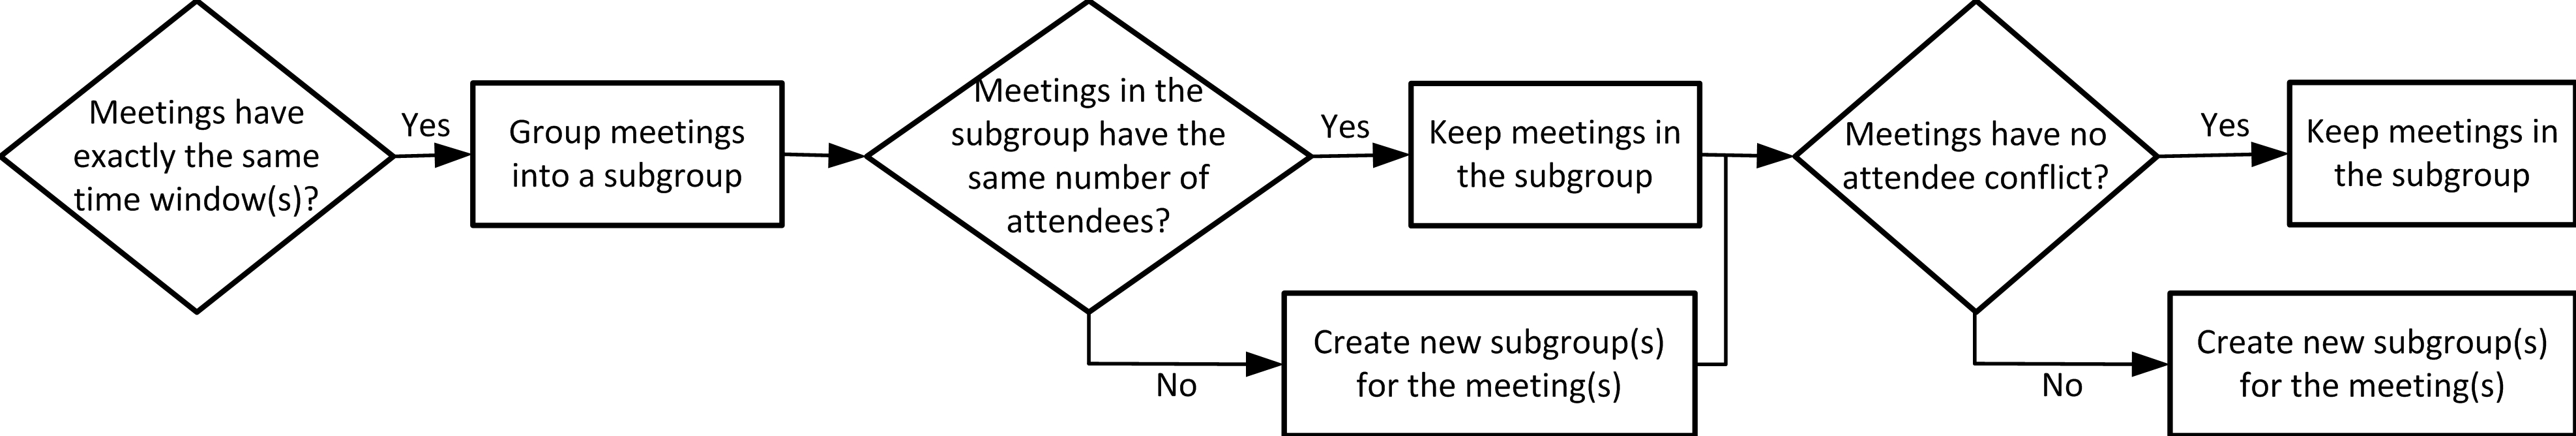
\includegraphics[width=1\linewidth]{figs/lns_mtype.jpg}
	\caption{The process flow of grouping identical meetings with similar properties.}
	%\vspace*{-2ex}
	\label{fig:mtype}
\end{figure}

One issue with the current model is that it can have a large number of equivalent solutions when two or more meetings are identical. In particular, let meetings 1 and 2 have the same time windows, same number of attendees, and no meeting conflicts. In this case, a solution in which $x_{1,l,k} = 1$ and $x_{2,l,k} = 0$ would be equivalent to one in which $x_{1,l,k} = 0$ and $x_{2,l,k} = 1$. In order to avoid the computational cost of generating both solutions we reduce the number of integer variables by defining meeting types. Meetings that are identical are considered to be of the same meeting type. Figure \ref{fig:mtype} illustrates the process flow of grouping meetings with similar properties into the same meeting type. Each subgroup represents a meeting type. Since the number of meeting types is smaller than the number of meetings, it allows for a simplified model that reduces symmetry. Without changing the model in its entirety we simply redefine $M$ to be the set of meeting requests and replace Constraint \eqref{eq:ms_every} with the one below to state that all meeting types must be scheduled $\psi_m$ times, where $\psi_m$ represents the number of meetings of type $m$.

\begin{equation} \label{eq:ms_everytype}
\mathop{\sum \limits_{l\in L_m, k \in K_m}} x_{m,l,k}= \psi_m \quad \forall m \in M
\end{equation}

%\noindent With constraints \eqref{eq:ms_everytype}, we remove the symmetries in meetings by grouping meetings of similar properties into single meeting type. 

\subsubsection{Simplifying The Building Thermal Dynamics Model}

The most involved constraints in the HVAC model come from modeling building thermal dynamics. In Section \ref{mip:thermal}, the temperature in a zone is affected by both internal and external walls. In our experiments, however, we observed that the temperature in a zone is mostly affected by the heat flow through external walls, the HVAC intervention and the occupants' heat load in the zone. The heat transfer from neighboring rooms through the internal walls is negligible based on our building settings. Hence, in our LNS model we only consider external walls, that is, those with that are outside facing. This approximation does not affect the HVAC control, hence it also does not impact the energy consumption, and therefore it does not impose any change to the schedule optimisation.
With this reduced model, the temperature constraints are simplified as follows:

\begin{equation}
\begin{split}
\begin{bmatrix}
\dot{T}_{l,k} \\
\dot{T}^{1}_{l,k} \\
. \\
. \\
\dot{T}^{N}_{l,k} \\
\end{bmatrix}
=
\begin{bmatrix}
-\frac{1}{\bm{C_l}} ( \sum_{n=1}^N \frac{1}{\bm{R_l^n}} + \frac{1}{\bm{R_l^w}}) & \frac{1}{\bm{C_l} \bm{R_l^1}} & . & . & \frac{1}{\bm{C_l} \bm{R_l^n}} \\
\frac{1}{\bm{C_l^1} \bm{R_l^1}} & -\frac{1}{\bm{C^1_l}} ( \frac{1}{\bm{R_l^1} + \bm{R_1^l}}) & 0 & 0 & 0 \\
. & . & . & . & .\\
. & . & . & . & .\\
\frac{1}{\bm{C_l^N} \bm{R_l^n}} & 0 & 0 & 0 & -\frac{1}{\bm{C^N_l}} ( \frac{1}{\bm{R_l^n} + \bm{R_N^l}})
\end{bmatrix}
\begin{bmatrix}
T_{l,k-1} \\
{T}^{1}_{l,k-1} \\
. \\
. \\
{T}^{N}_{l,k-1} \\
\end{bmatrix}
\\ +
\begin{bmatrix}
\frac{1}{\bm{C_l} \bm{R_l^w}} &
0 &
\frac{1}{\bm{C_l}}
\\
\frac{1}{\bm{C_l^1} \bm{R^l_1}} &
\frac{1}{\bm{C_l^1}} &
0 \\
. & . & . \\
. & . & . \\
\frac{1}{\bm{C_l^N} \bm{R^l_N}} &
\frac{1}{\bm{C_l^N}} &
0
\end{bmatrix}
\begin{bmatrix}
T^{OA}_{k-1} \\
Q^s_{l,k-1} \\
Q^p_{l,k-1}
\end{bmatrix}
+
\begin{bmatrix}
\frac{\Delta H^l_{k-1}}{\bm{C_l}} \\
0 \\
. \\
. \\
0
\end{bmatrix}
\end{split} \label{eq:roomtemperature_lns}
\end{equation}
%\begin{equation}
%Q^p_{l,k} = q^p pp_{l,k} \quad \forall l \in L, k \in K \label{eq:occupants}
%\end{equation}
%\begin{equation}
%\Delta H_{l,k} = C^{pa} a^{SA}_{l,k} (T^{SA}_{l,k} - T_{l,k}) \quad \forall l \in L, k \in K \label{eq:enthalpy}
%\end{equation}

Constraints \eqref{eq:roomtemperature_lns} model the temperature dynamics in zone $l$ when considering a room with $N$ external walls.  The expression $\dot{T}_{l,k} = \frac{T_{l,k} - T_{l,k-1}}{\bm{\Delta t}}$ is the rate of change in zone temperature and $\dot{T}^n_{l,k}$ is the rate of change in temperature of the external wall(s) $n = 1,..., N$. Recall that $\bm{C_l}$ and $\bm{C^N_l}$ respectively denote the thermal capacitance of zone $l$ and of the external wall $n$ in zone $l$. $\bm{R^n_l}$ and $\bm{R^w_l}$ respectively represent the thermal resistance of wall $n$ and the windows separating zone $l$ with the outdoors. $\bm{T^{OA}$} is the outdoor temperature, while $Q^s$ is the solar heat gain. With this, the building thermal dynamics model is obtained by adding equations \eqref{eq:roomtemperature_lns} with equations \eqref{eq:heatgain}, \eqref{eq:enthalpy}, \eqref{eq:tlf} and \eqref{eq:tlc}


\subsection{Summary of Model Equations}

\noindent \emph{GenInitialMeetingSchedule}. The initial schedule is generated by combining Equations \eqref{eq:objective_minr}, \eqref{eq:ms_minroomalloc}, \eqref{eq:ms_everytype}, and \eqref{eq:ms_totalalloc}-\eqref{eq:ms_meeting}.

\vspace{2pt}
\noindent \emph{GenHVACControl}.  The initial HVAC control is generated by adding Equations \eqref{eq:objective} - \eqref{eq:aSAT4}
with Equations~\eqref{eq:p_heat} and Equations~\eqref{eq:enthalpy} being linearised. Also, Equations \eqref{eq:roomtemperature}, \eqref{eq:temp:outer} and \eqref{eq:temp:inner} are replaced by \eqref{eq:roomtemperature_lns}. The result from the initial schedule, that is the values of $x_{m,l,k}$, is set as an input to this model. 

\vspace{2pt}
\noindent \emph{RepairNeighborhood}. The MIP model is formed by limiting $l$ to the selected neighbourood $L'$, and run the joint HVAC control and occupancy scheduling model by combining Equations \eqref{eq:objective}-\eqref{eq:hvac_standby_ASA}, \eqref{eq:roomtemperature_lns}, \eqref{eq:heatgain}-\eqref{eq:enthalpy}, \eqref{eq:tlf}-\eqref{eq:aSAT4}, \eqref{eq:ms_everytype}, \eqref{eq:ms_totalalloc}-\eqref{eq:ms_meeting}.


\section{Experiments}\label{sec:results}

\subsection{MIP vs. LNS}

\begin{figure}
	\centering
		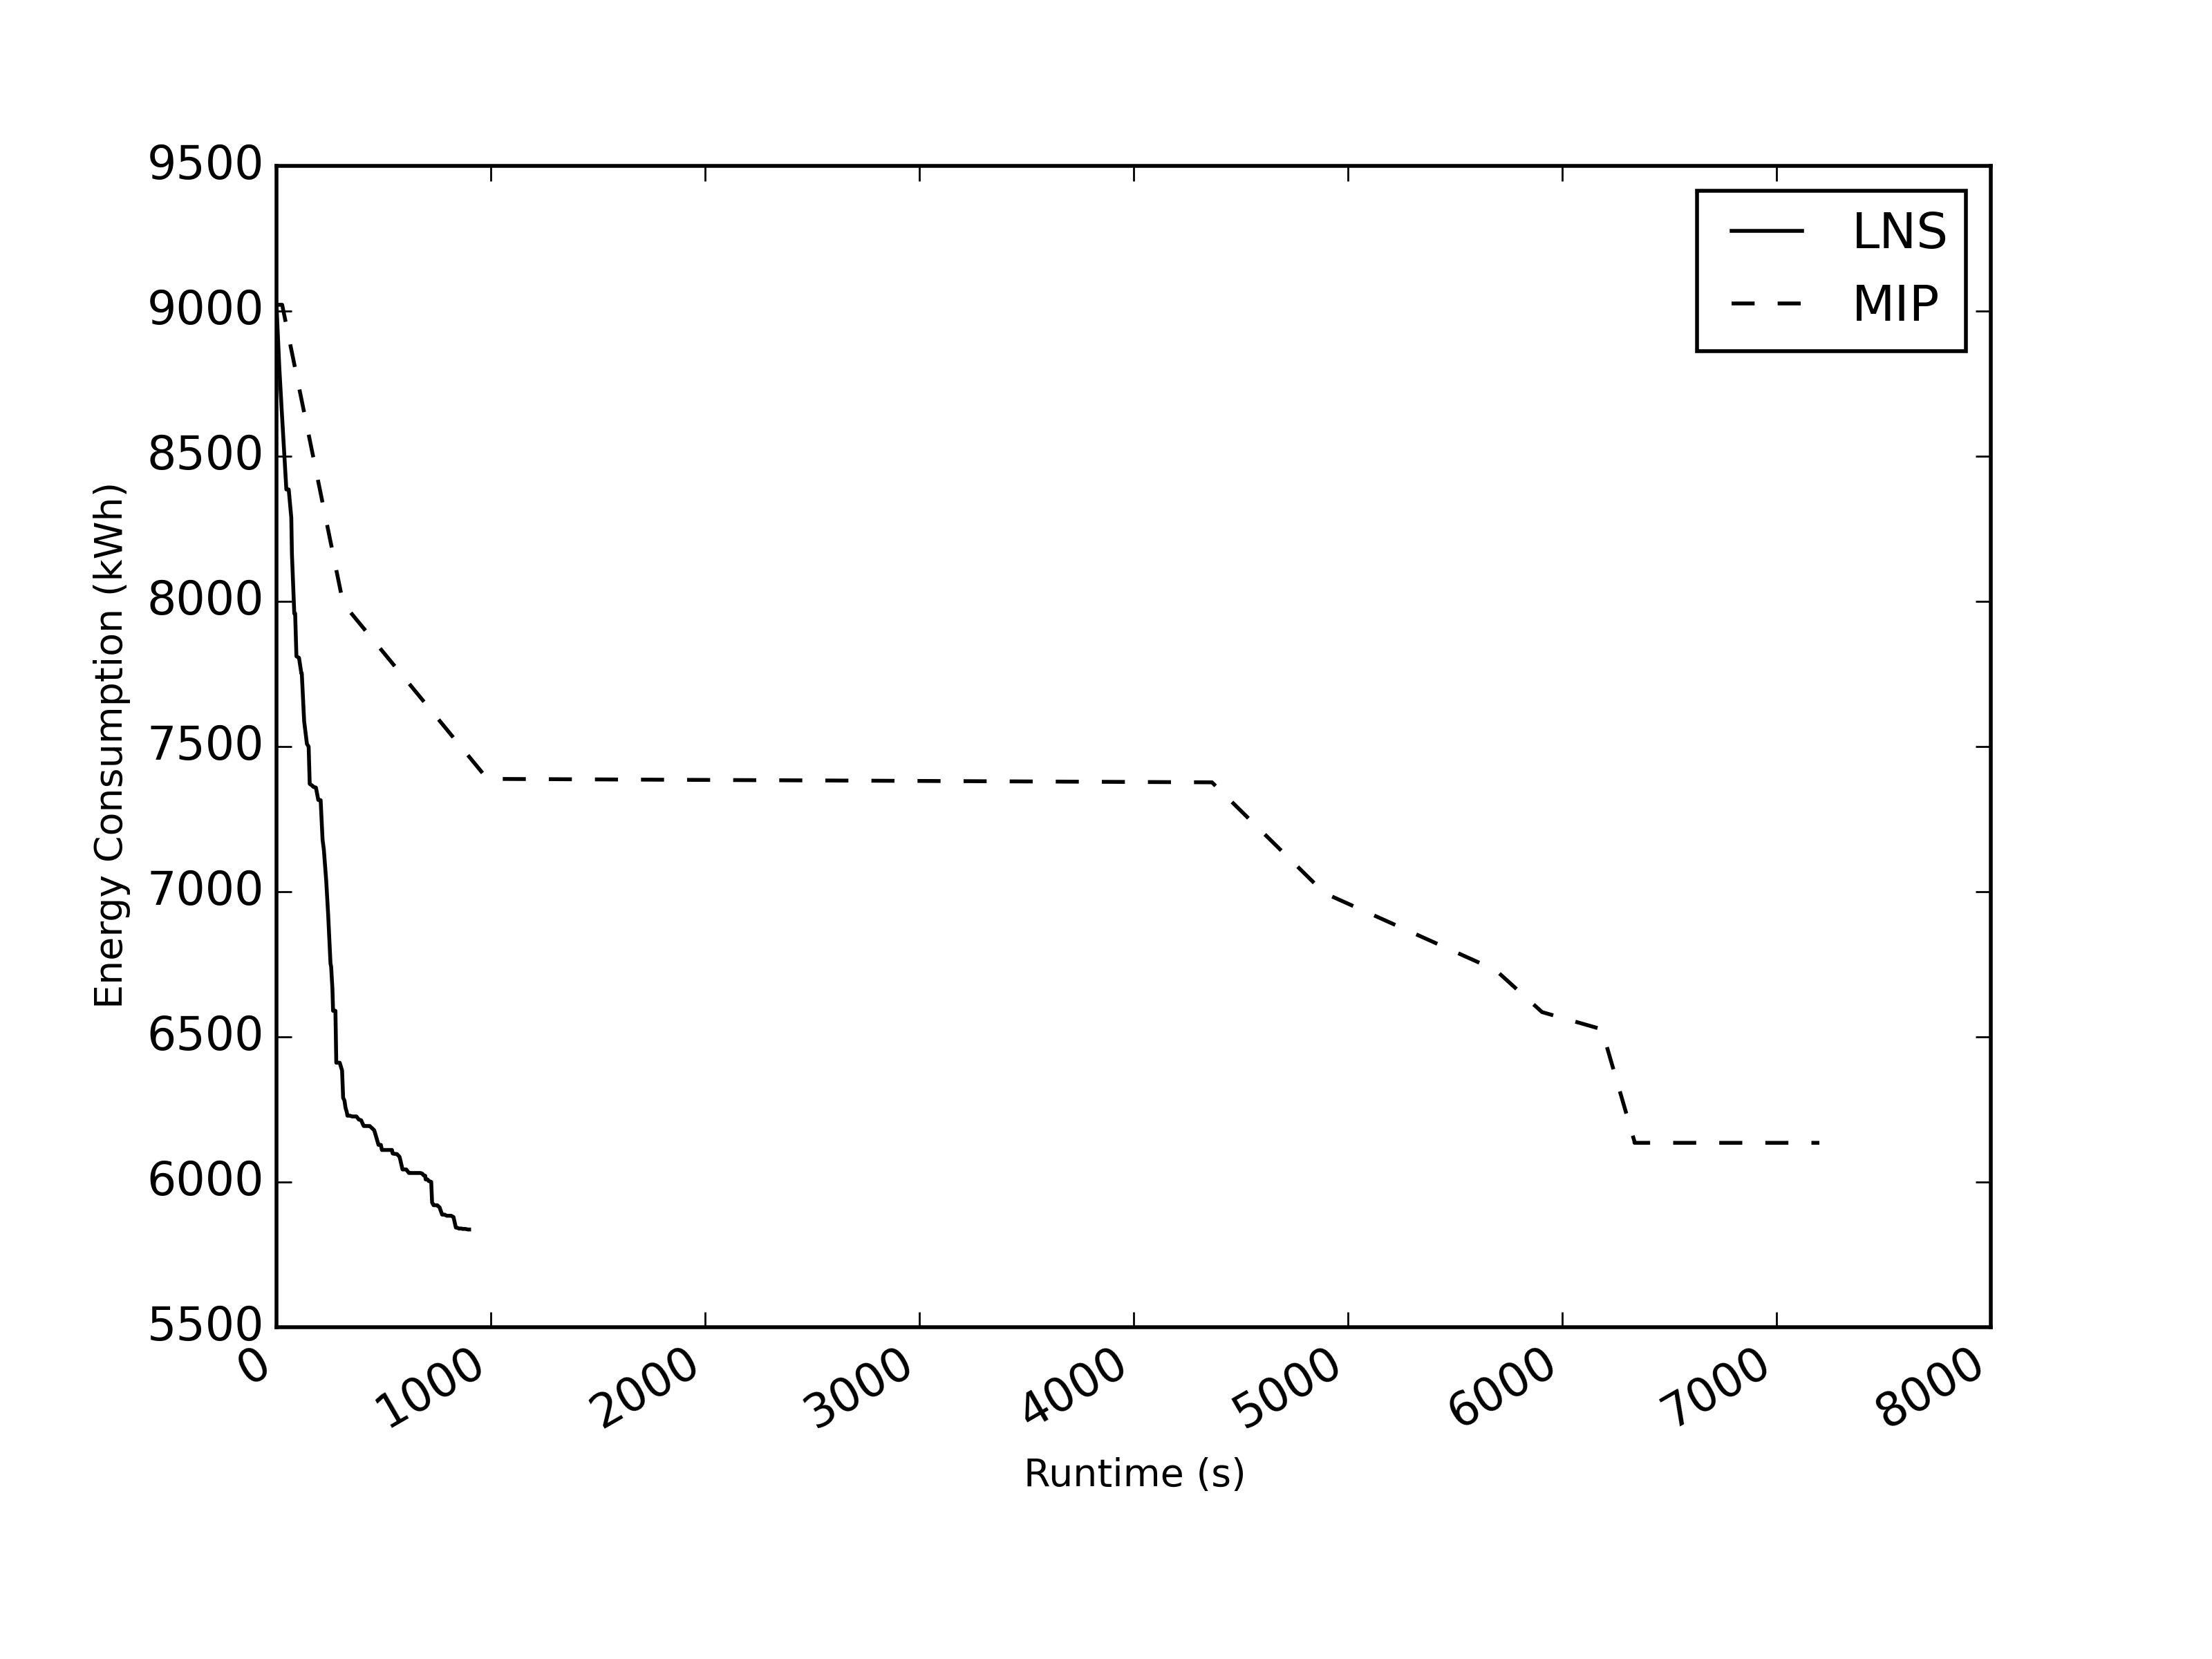
\includegraphics[width=0.9\linewidth]{figs/eams_meeting_m200_2.png} \\
(a) Instance 1  \\[6pt]
		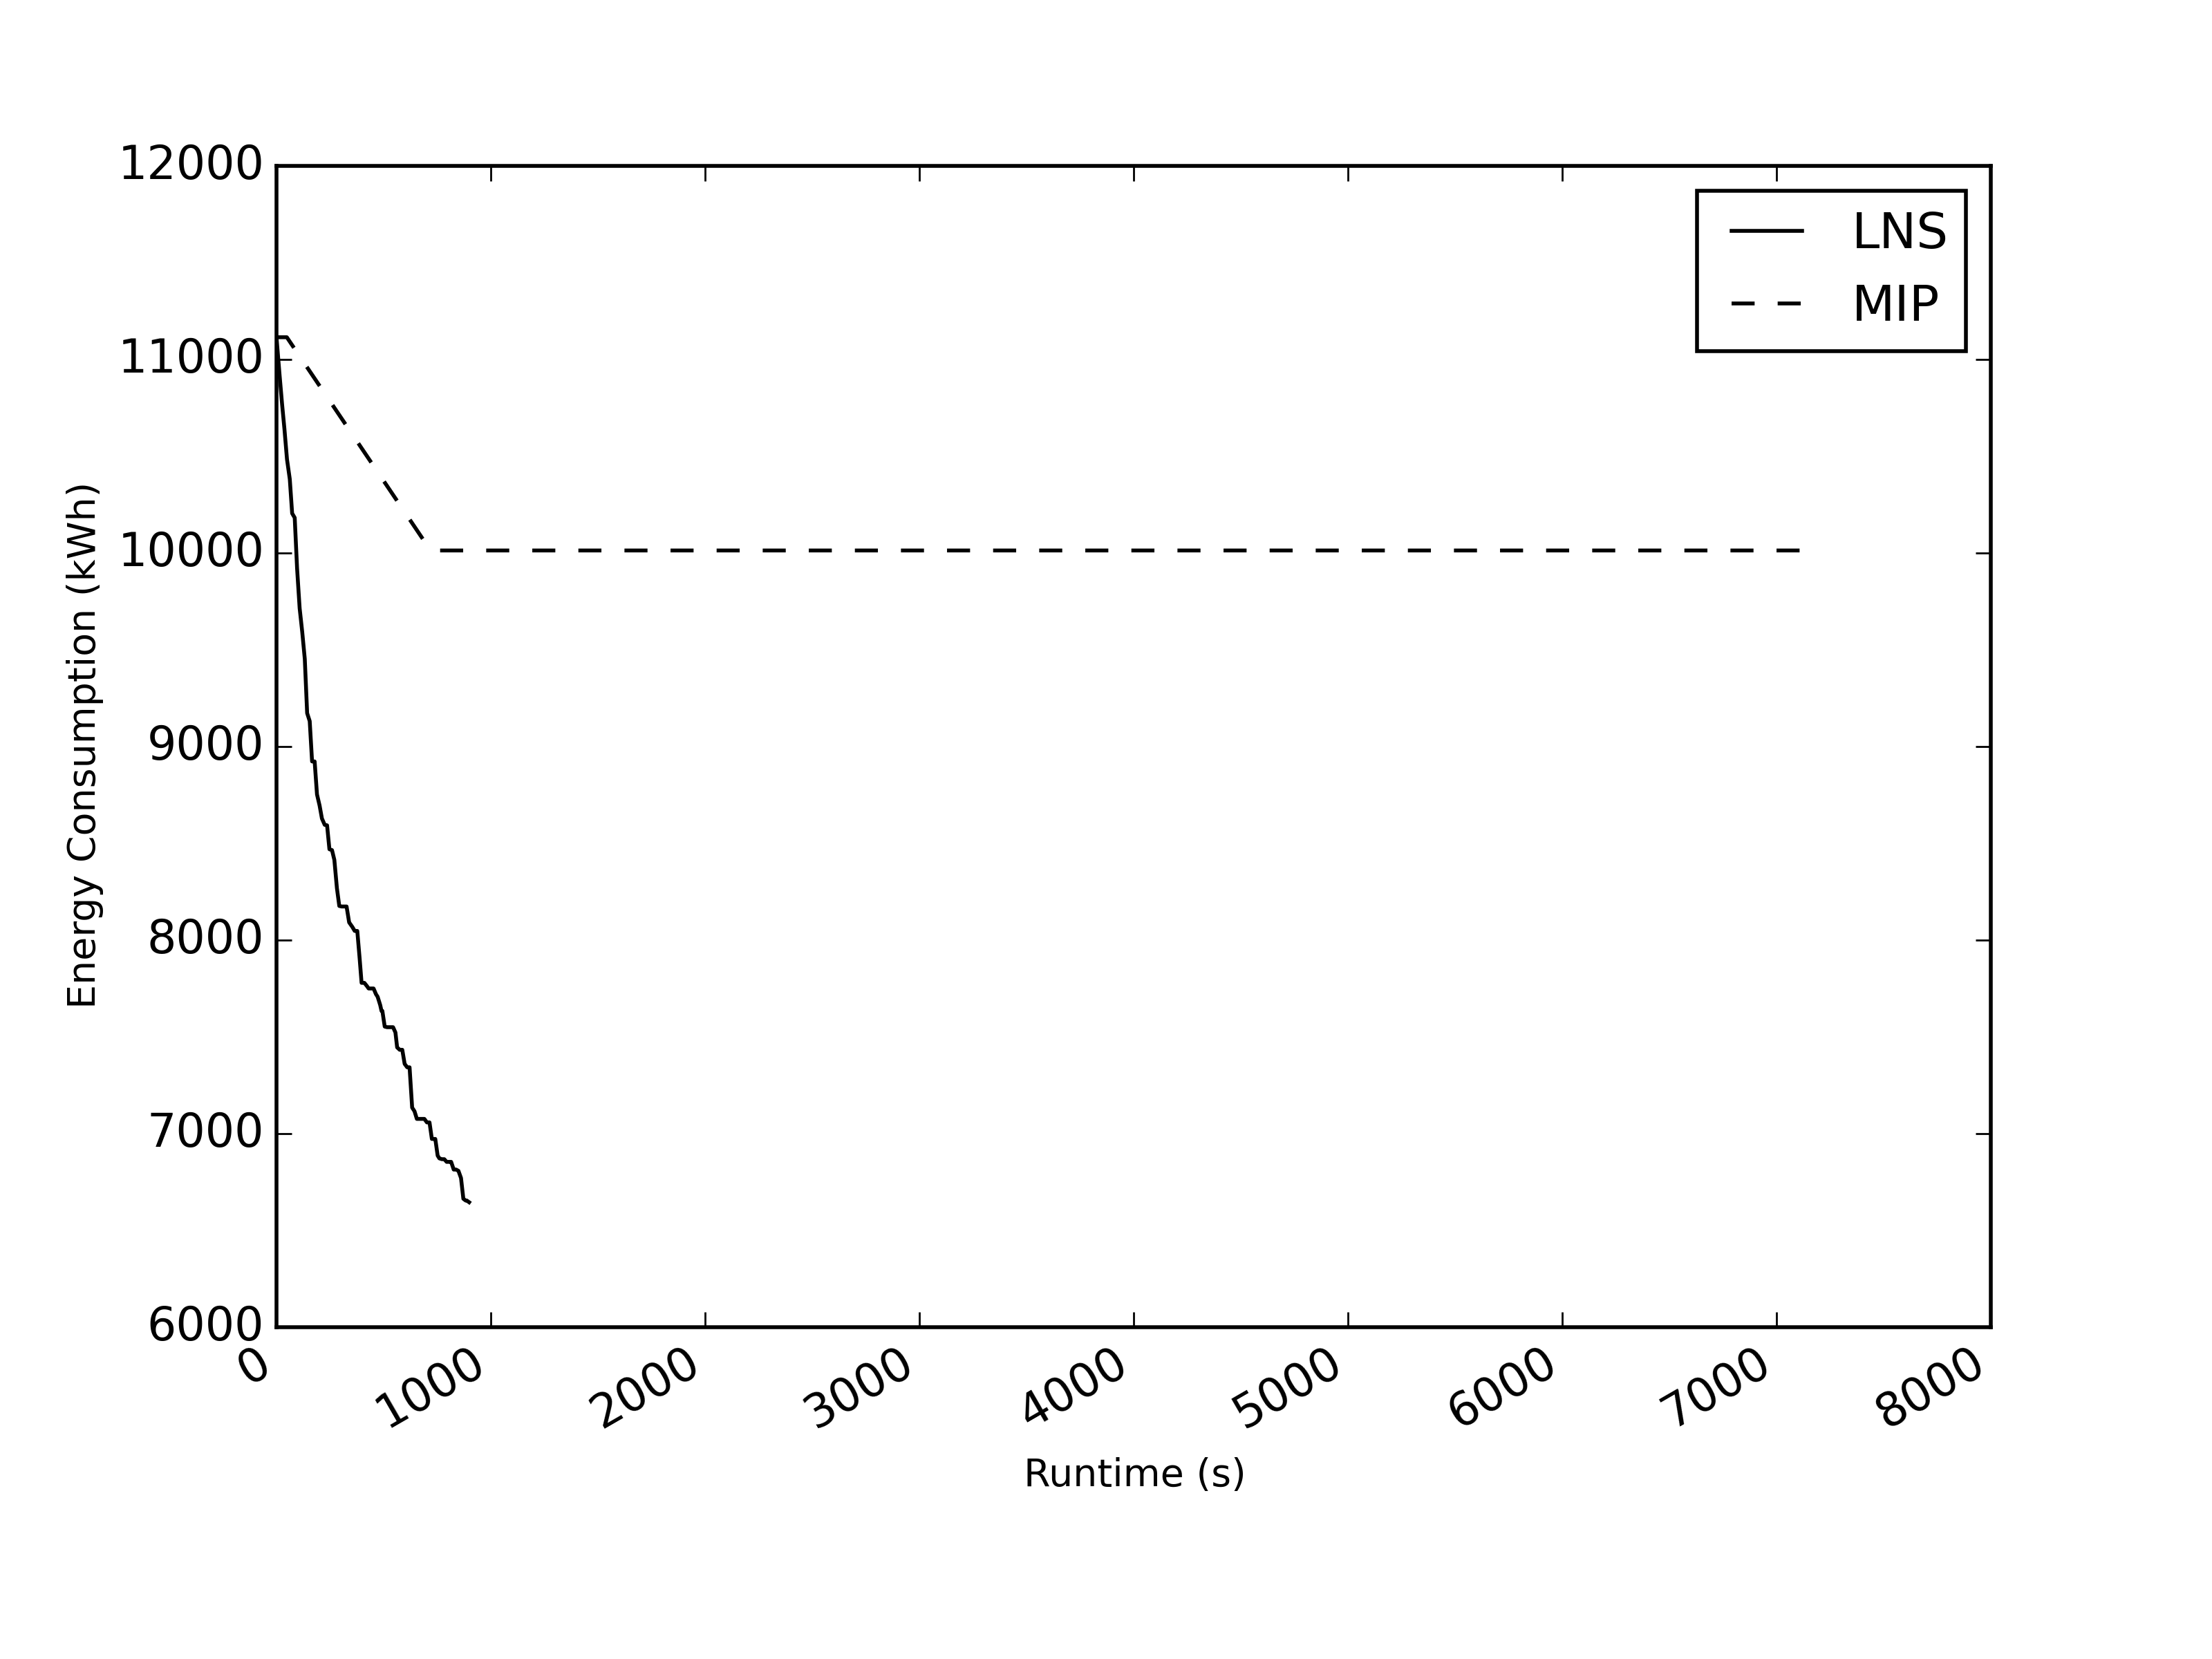
\includegraphics[width=0.9\linewidth]{figs/eams_meeting_m200_1.png}\\
(b) Instance 2  \\[6pt]
	\caption{Typical performance of MIP (2 hours) and LNS (15 minutes) on two benchmark instances.}
	\label{fig:compare}
\end{figure}

Before describing our main results, we first point out the typical behavior of solving energy aware meeting scheduling as a MIP. Figure \ref{fig:compare} shows the performance of the MIP approach on two typical problem instances when given 2 hours of runtime. In general, MIP's convergence on large problems is slow and sometimes MIP fails to converge even after 2 hours. This is exactly why we developed the LNS approach. The typical performance of the LNS approach is also given in Figure \ref{fig:compare}. In the figure, LNS was given only 15 minutes of runtime but it is capable of returning significantly better results when compared to MIP.



\subsection{Combining MIP with LNS}\label{sec:lns_eg}

\begin{figure}
	\centering
		\includegraphics[width=0.9\linewidth]{figs/lns_sche_init1.jpg} \\
(a) Initial schedule  \\[6pt]
		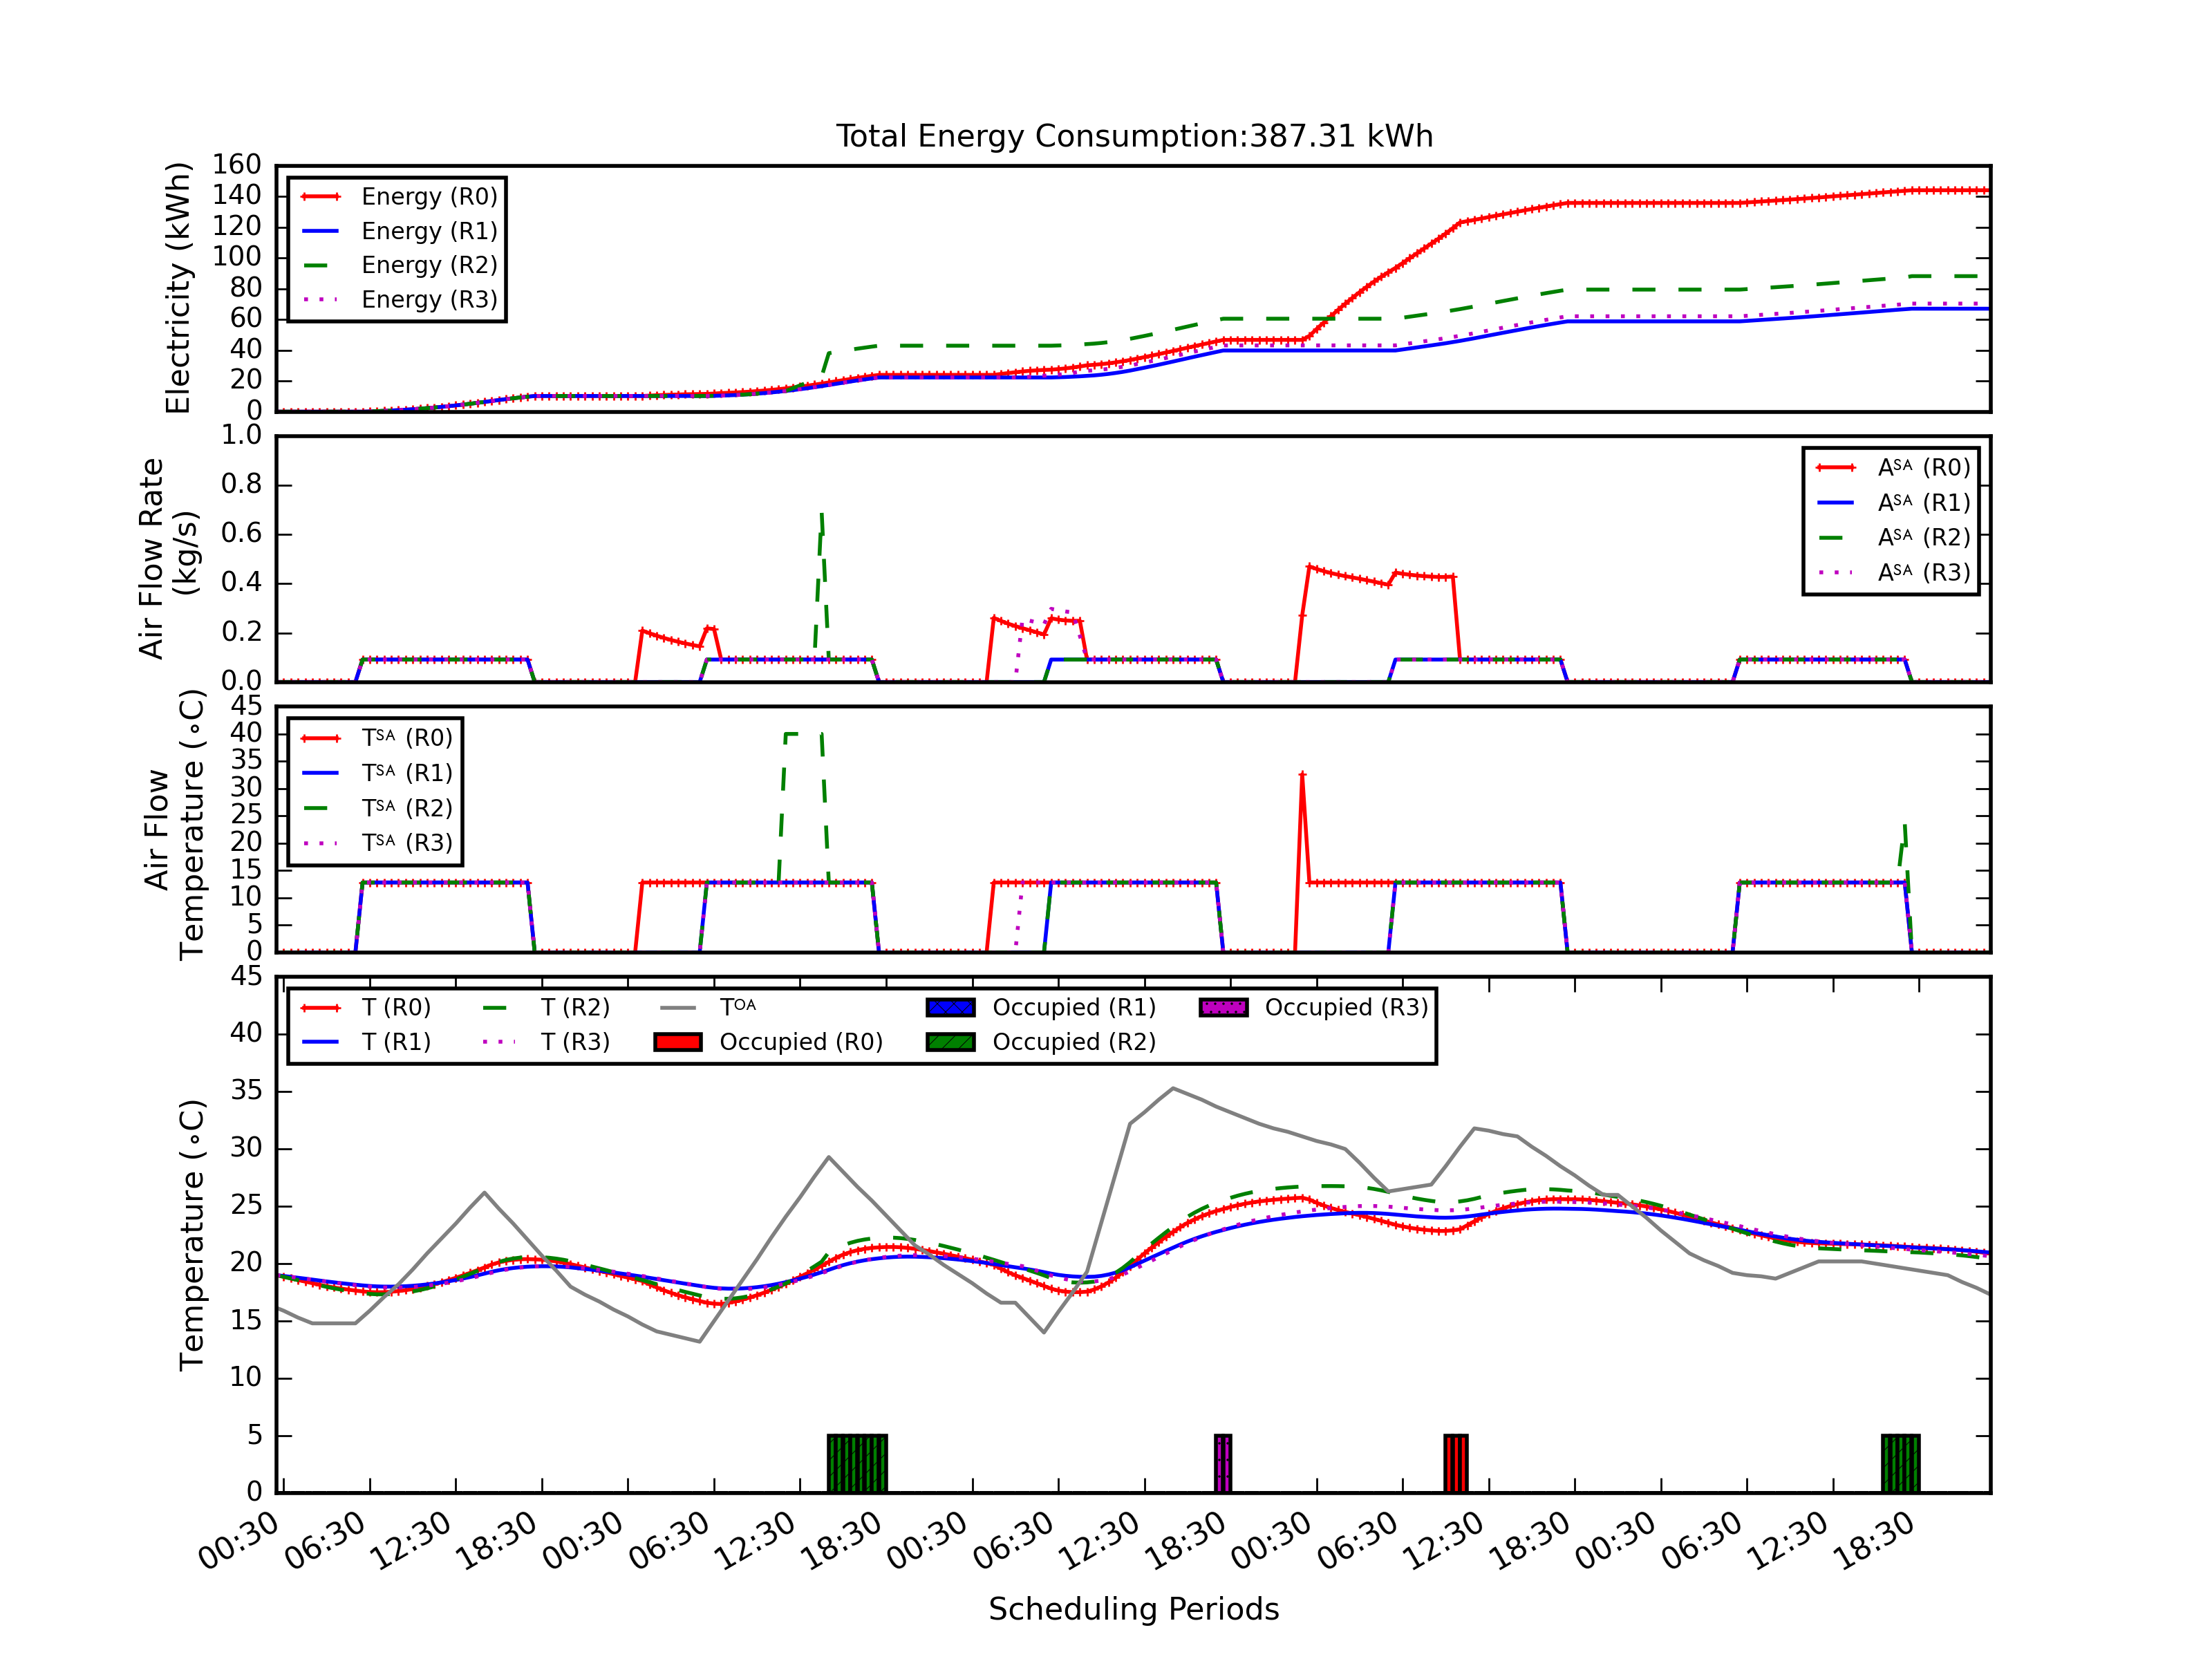
\includegraphics[width=1\linewidth]{figs/lns_init.png}\\
(b) HVAC control for Room R0-R3  \\[6pt]
	\caption{Large neighbourood search - initial schedule}
	\label{fig:lns_init}
\end{figure}

Figure \ref{fig:lns_init}--\ref{fig:lns_dr3} illustrate a high-level scenario example of our large neighbourhood search approach. These figures give an insight of how schedules are being initialized, destroyed and repaired over 5-days in 20 rooms using our LNS algorithm. In Figure \ref{fig:lns_init}(a), an initial schedule is generated by greedily scheduling all meetings in the minimum number of rooms each day. More rooms are used only if there are overlapping meetings that have to be scheduled in different locations. This schedule is then fed into our occupancy-based HVAC control model. Figure \ref{fig:lns_init}(b) shows the optimised HVAC control based on the given schedule. With this initialization approach, we can quickly generate an initial feasible schedule and an optimal HVAC control for large number of meetings and rooms. For simplicity, only the HVAC controls for room R0 to R3 are shown. Note that 1 slot in \ref{fig:lns_init}(a) is equivalent to 2 slots in \ref{fig:lns_init}(b), and the occupied slots are depicted as vertical blocks (30 minutes each) in the third subgraph of \ref{fig:lns_init}(b). 
% Standby mode is on, hence wwe see that the HVAc is activated in R0 and R3 during off peak hour to pre-cool the rooms.
% R2 is warmed up with high TSA.


\begin{figure}
	\centering
		\includegraphics[width=0.9\linewidth]{figs/lns_sche_ds1.jpg} \\
(a) Schedule: destroy \& repair room R0 and room R1 \\[6pt]		
		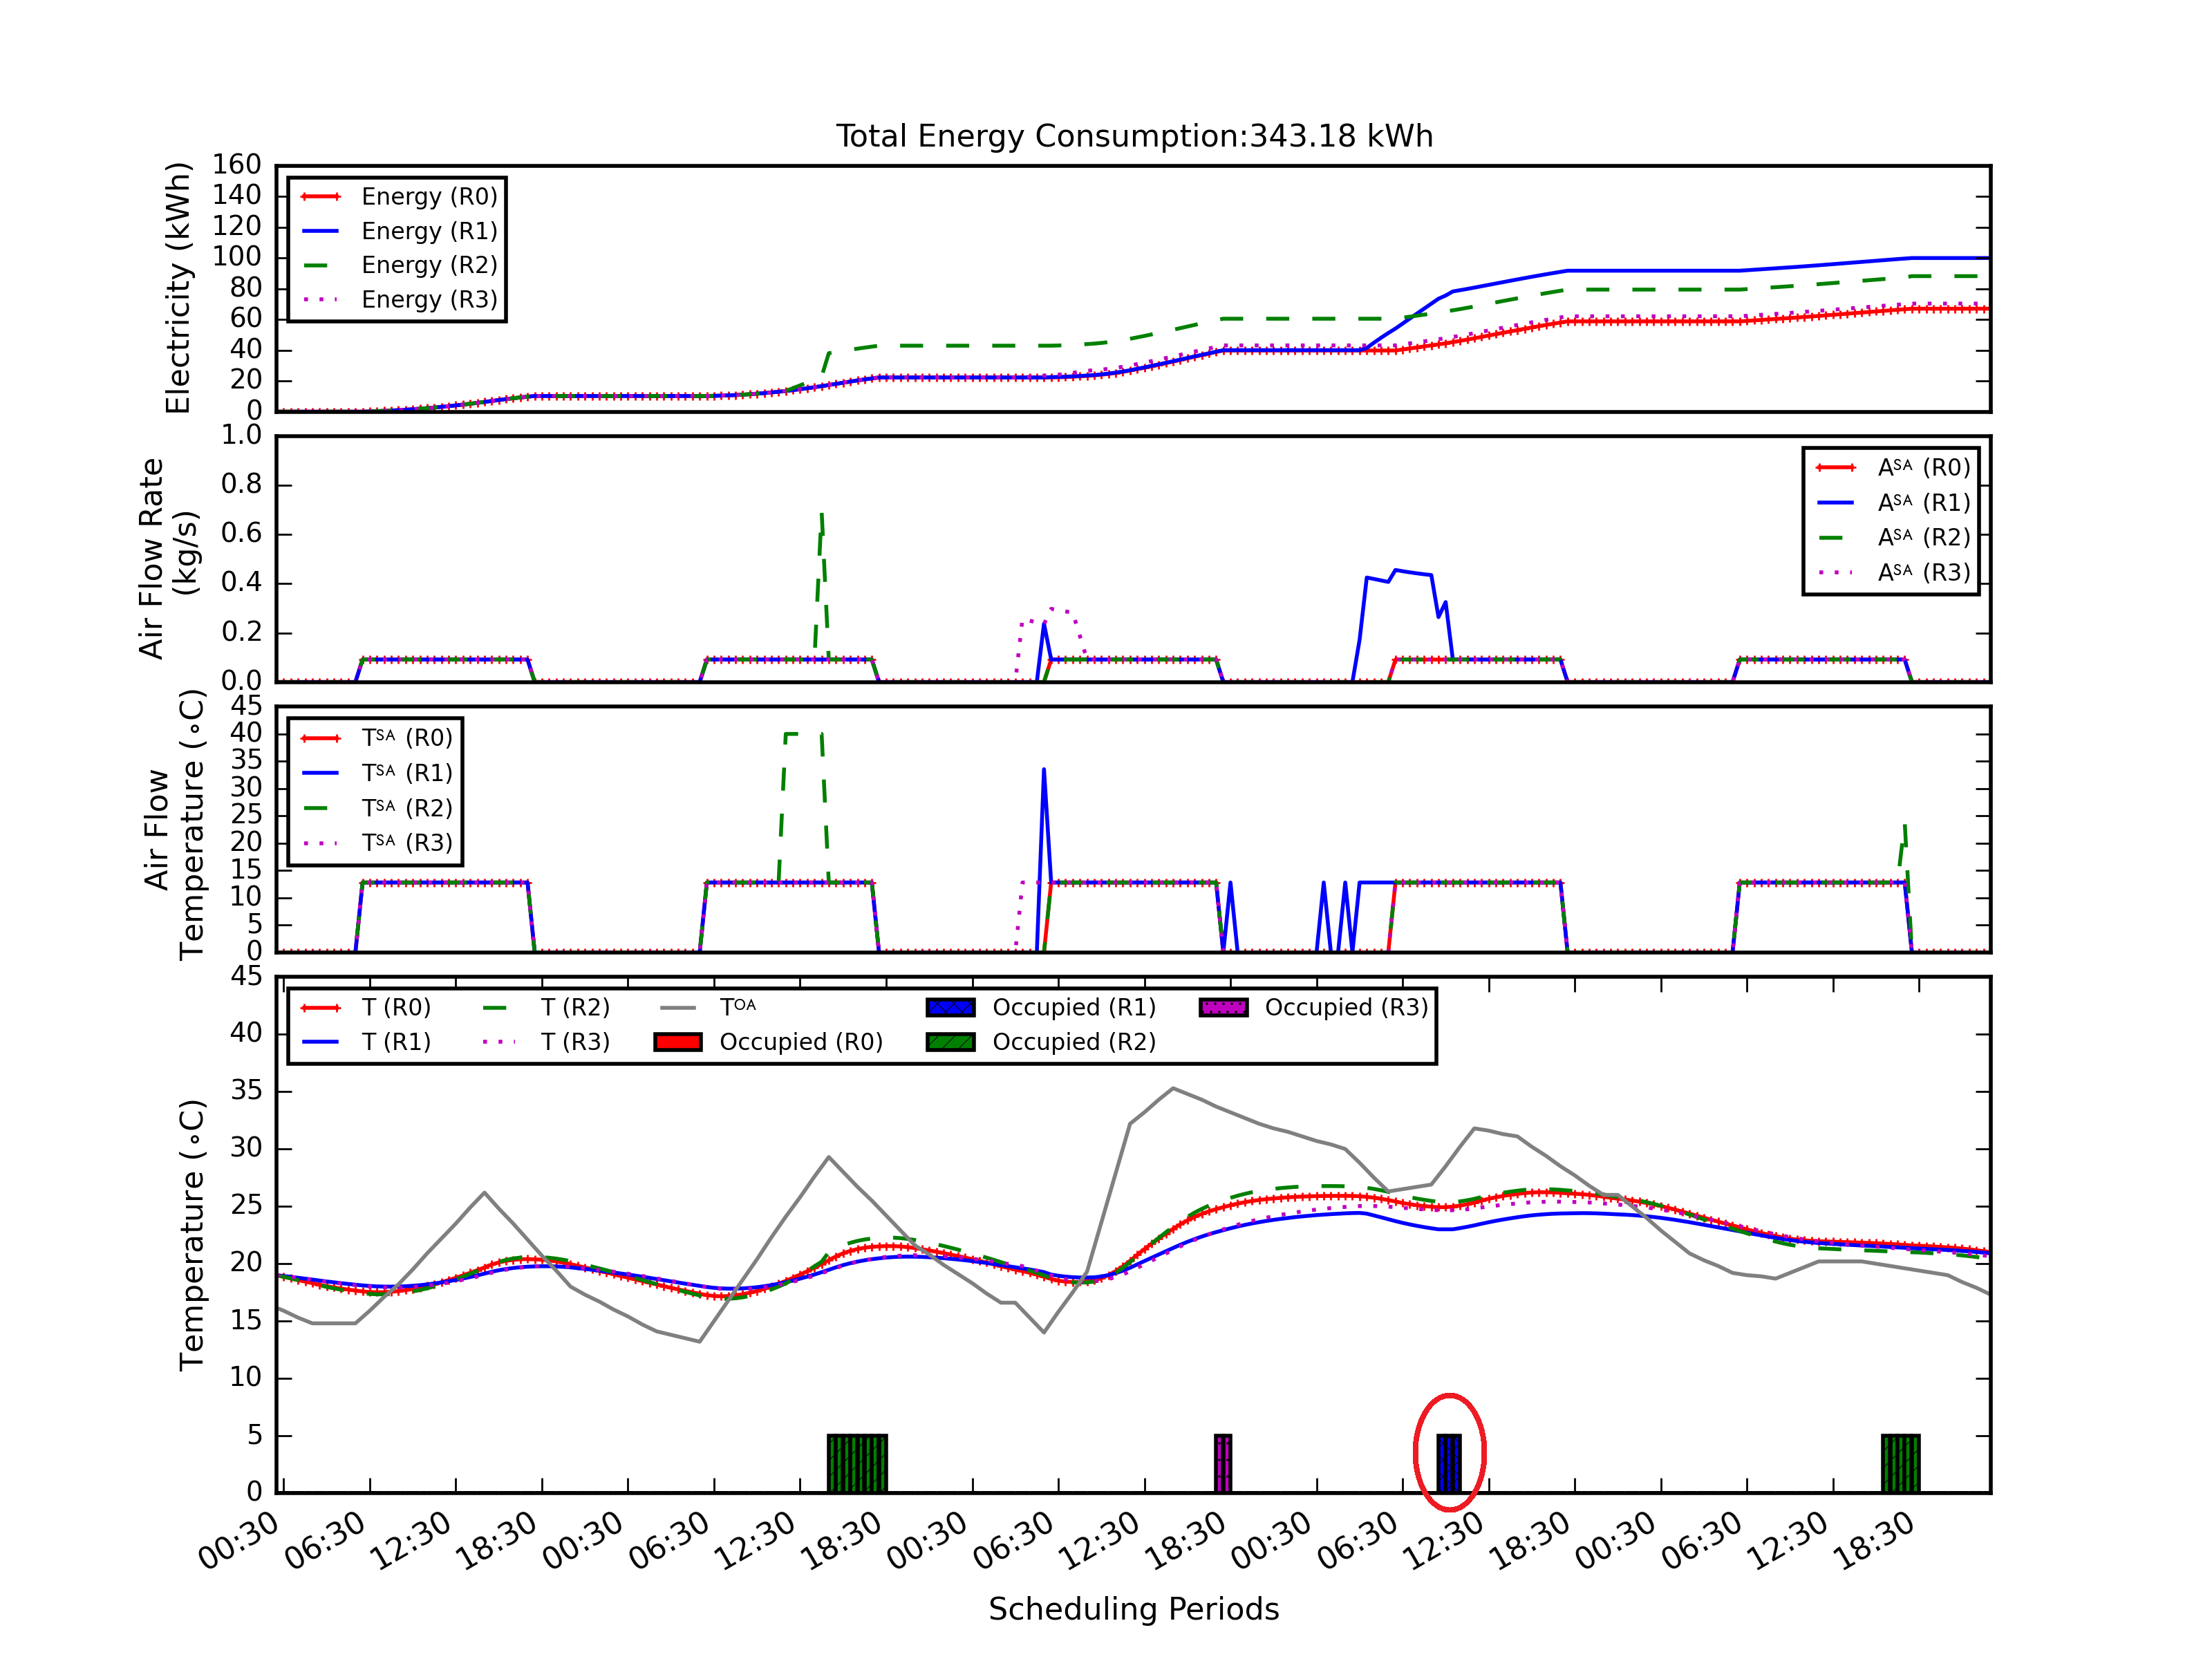
\includegraphics[width=1\linewidth]{figs/lns_dr1.png} \\
(b) HVAC control for Room R0-R3  \\[6pt]
	\caption{Large neighbourood search - iteration 1: destroy \& repair steps}
	\label{fig:lns_dr1}
\end{figure}

Figure \ref{fig:lns_dr1} depicts the first iteration of the destroy and repair step. In this iteration, Room R0 and Room R1 are randomly selected. All meetings scheduled in Room R0 and Room R1 are destroyed, and a schedule re-optimisation is executed. In this scenario, meetings in Room R0 are moved to Room R1, as shown in Figure \ref{fig:lns_dr1}(a). We observe from Figure \ref{fig:lns_dr1}(b) that this leads to a reduction of 44 kWh. %We observe from Figure \ref{fig:lns_dr1}(b) that this occurs as an energy reduction of 44 kWh can be achieved by simply swapping the meetings from room R0 to room R1.


\begin{figure}
	\centering
		\includegraphics[width=0.9\linewidth]{figs/lns_sche_ds2.jpg}\\
(a) Schedule: destroy \& repair room R0 and room R3  \\[6pt]
		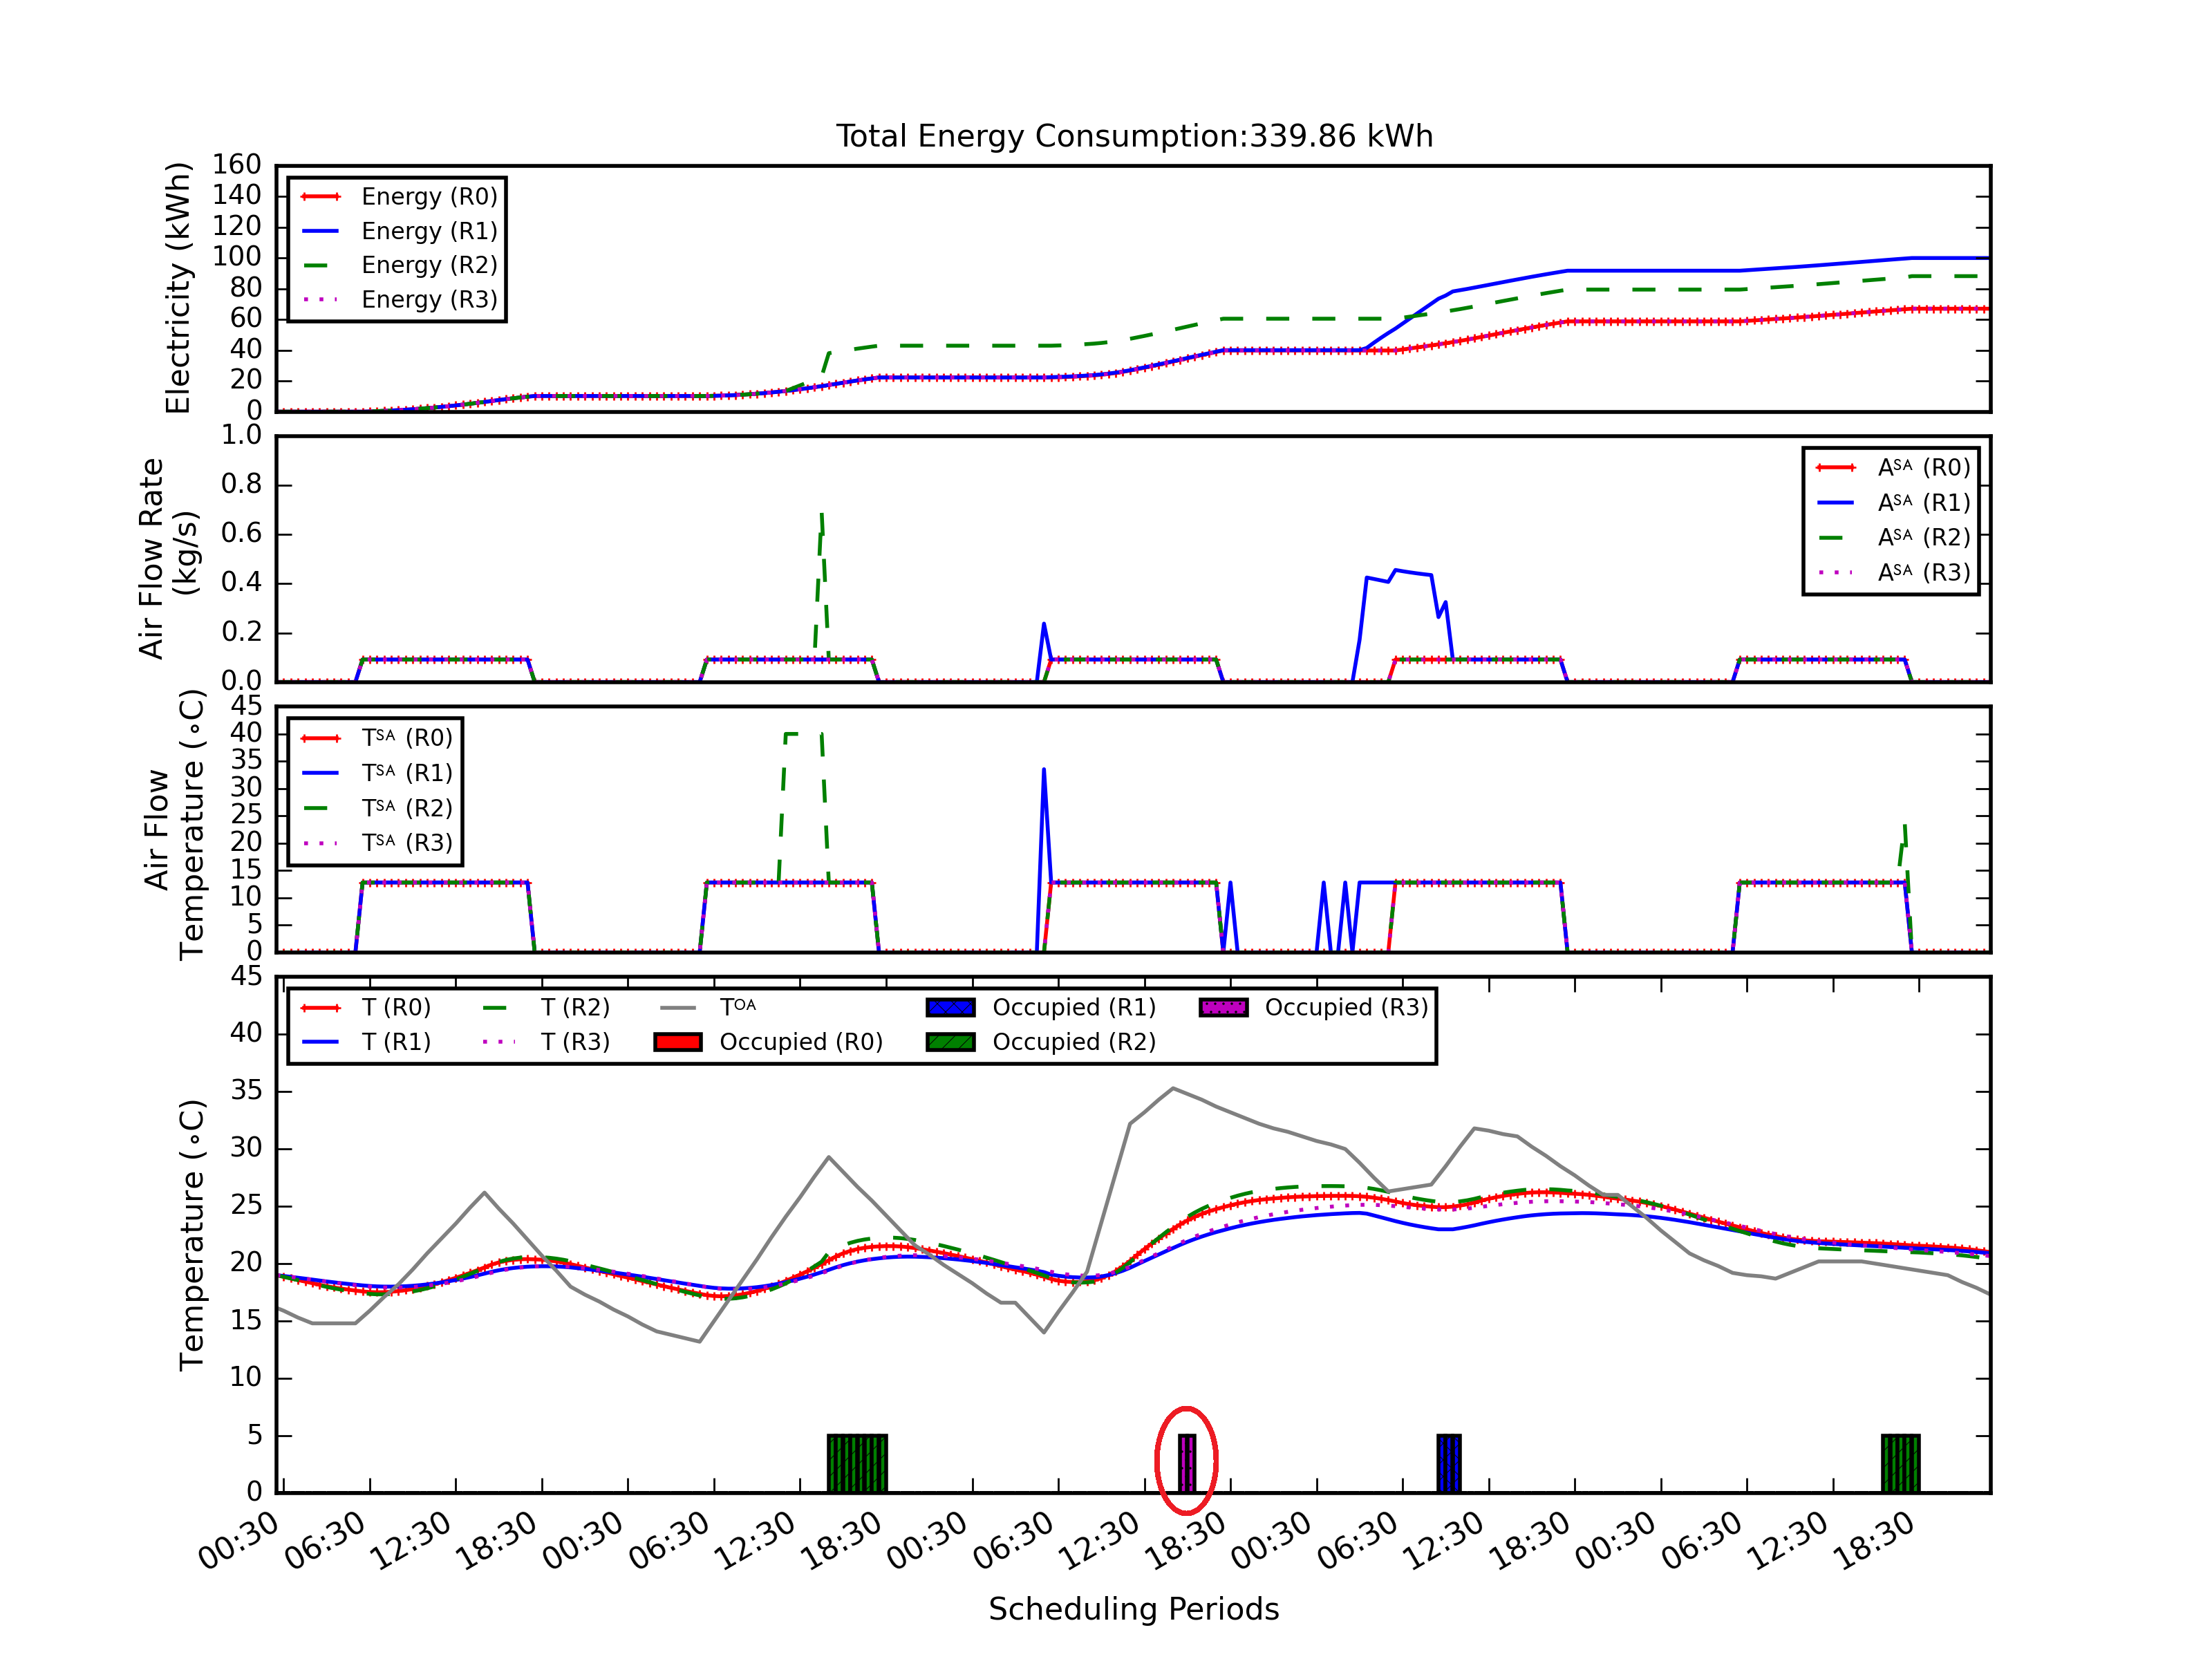
\includegraphics[width=1\linewidth]{figs/lns_dr2.png} \\
(b) HVAC control for Room R0-R3  \\[6pt]
	\caption{Large neighbourood search - iteration 2: destroy \& repair steps}
	\label{fig:lns_dr2}
\end{figure}

Figure \ref{fig:lns_dr2} presents the second iteration of destroy and repair step. In this round, Room R0 and Room R3 are selected. There is no meeting scheduled in R0 now. However, a better schedule is found by re-scheduling meetings in Room R3 to earlier time slots, as shown in Figure \ref{fig:lns_dr2}(a). Figure \ref{fig:lns_dr2}(b) reveals the reason behind this move. By moving the meetings 2.5 hours earlier, it helps to reduce the supply air flow rate required to maintain the room temperature at comfort bounds, as that day has relative high outdoor temperature. By doing this, a 3.32kWh of energy is saved.


\begin{figure}
	\centering
		\includegraphics[width=0.9\linewidth]{figs/lns_sche_ds3.jpg}\\
(a) Schedule: destroy \& repair room R0 and room R2  \\[6pt]
		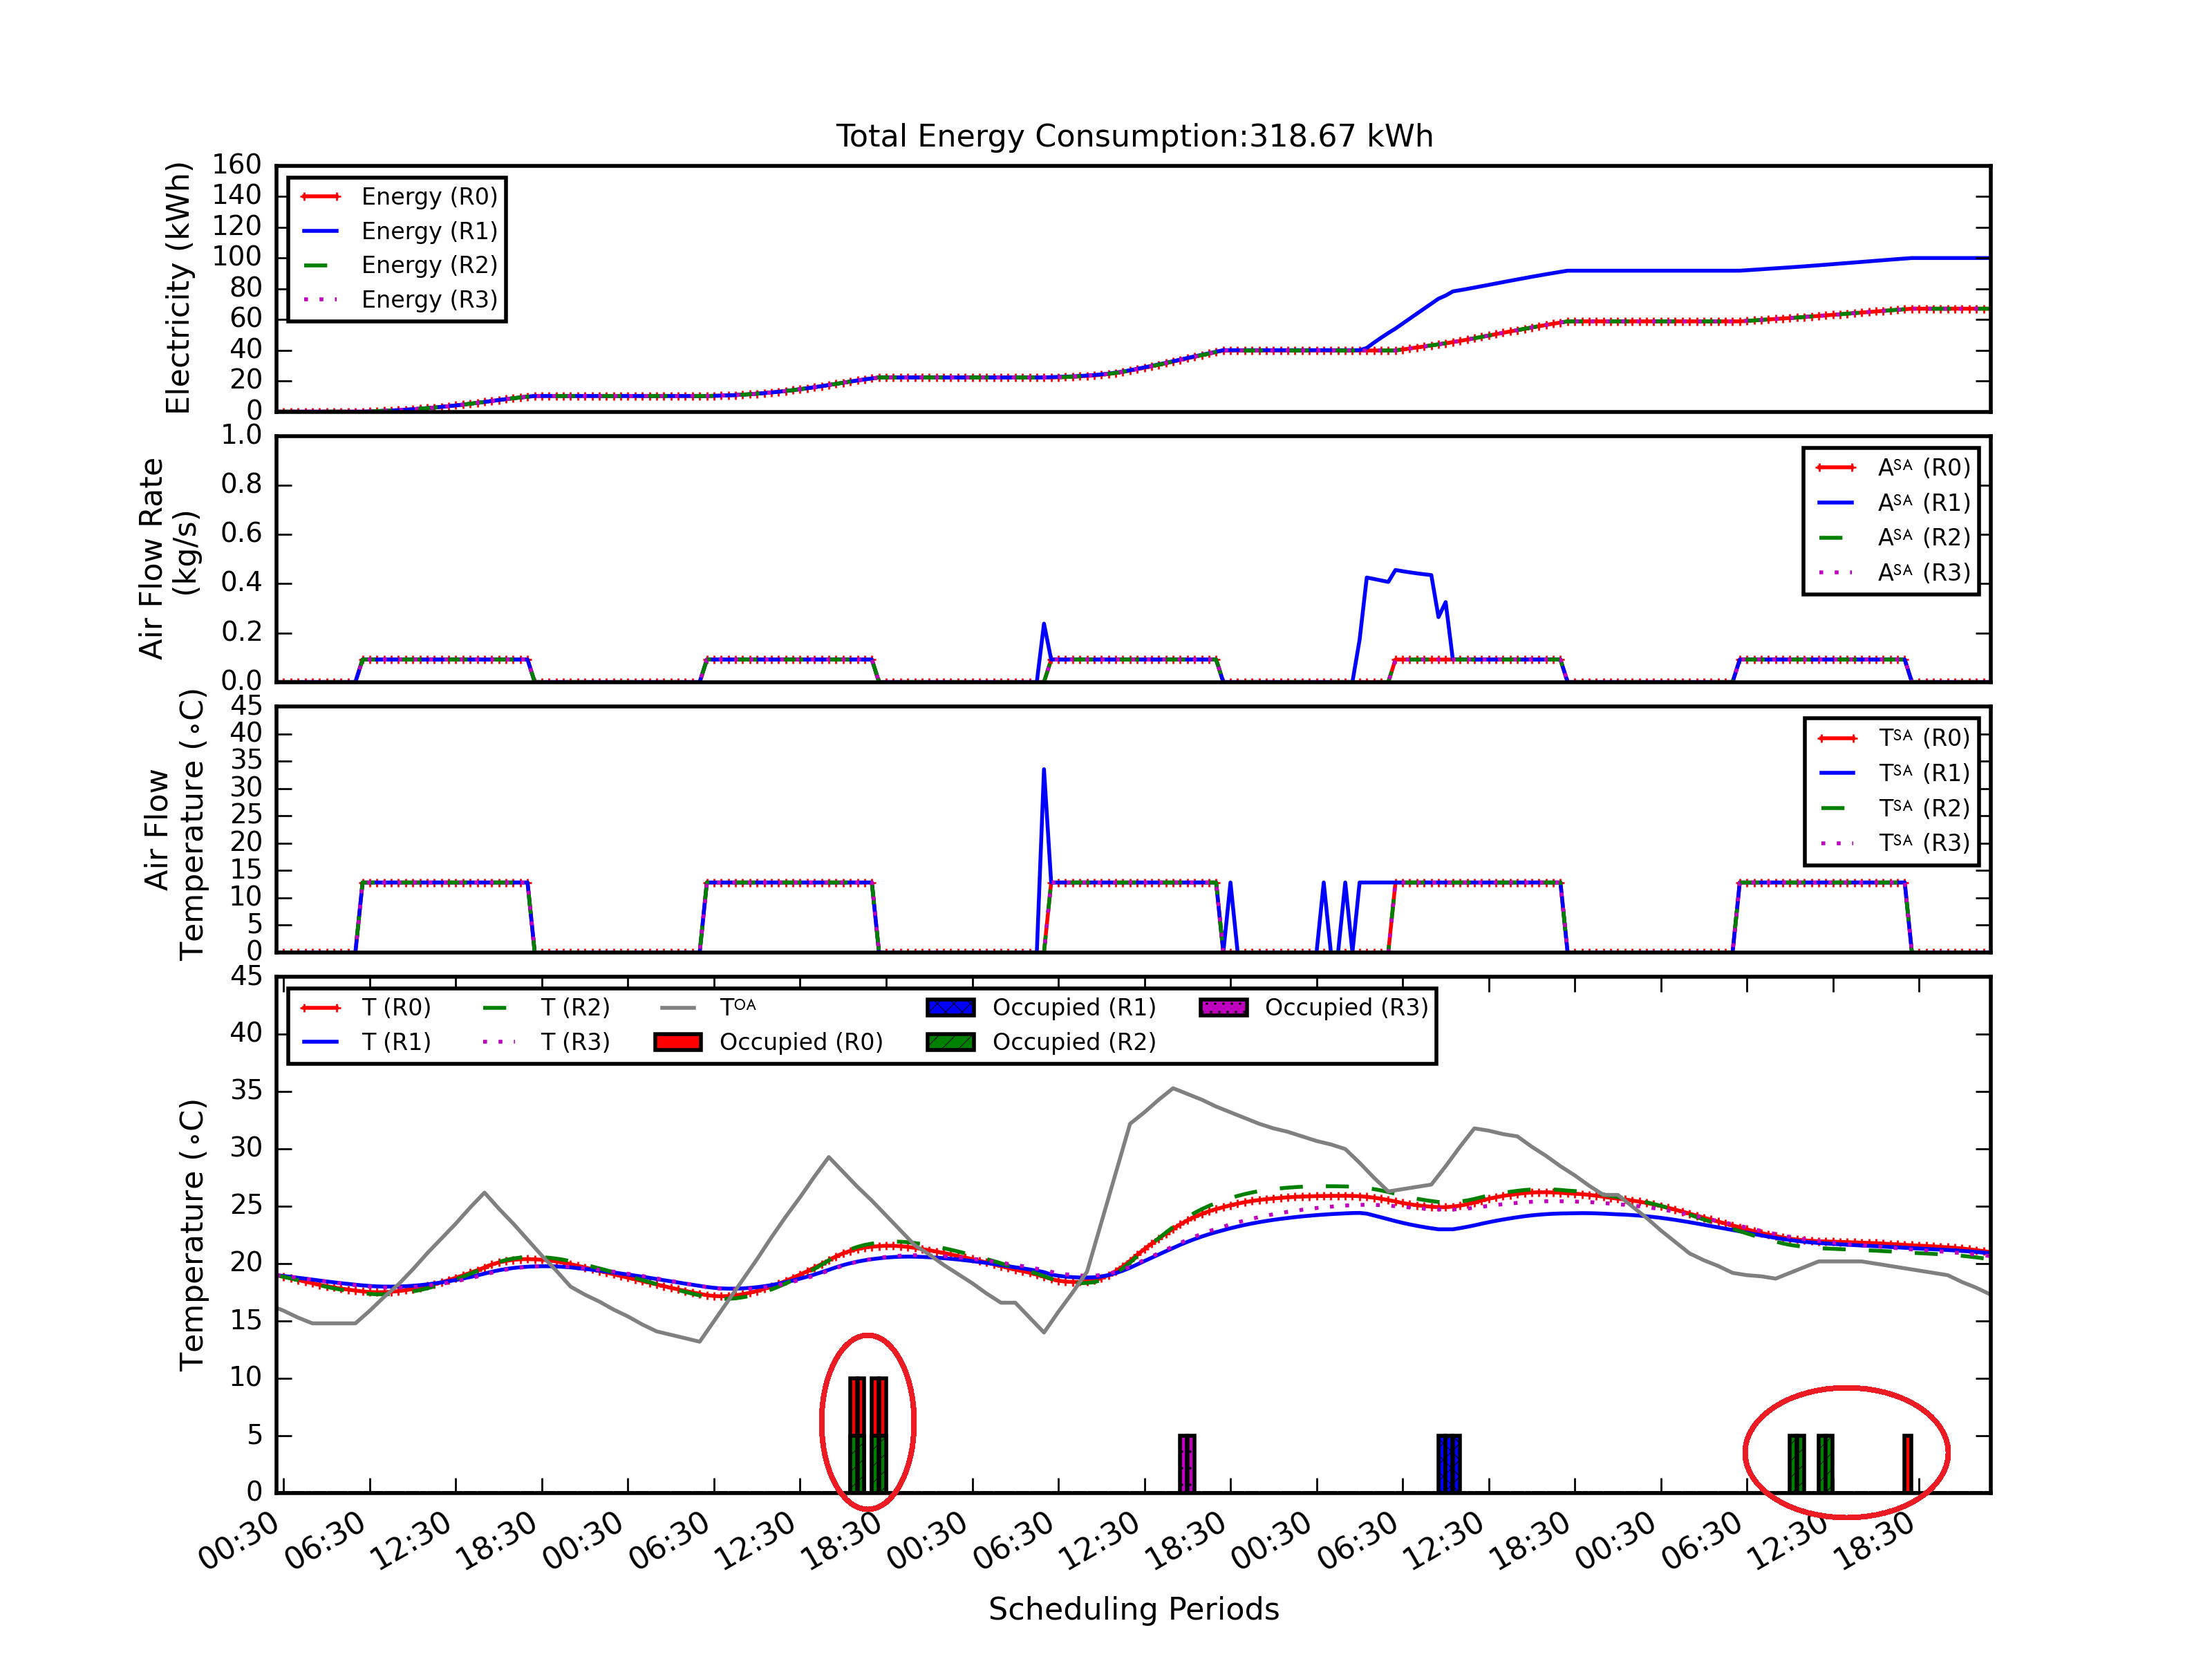
\includegraphics[width=1\linewidth]{figs/lns_dr3.png} \\
(b) HVAC control for Room R0-R3  \\[6pt]
	\caption{Large neighbourood search - iteration 3: destroy \& repair steps}
	\label{fig:lns_dr3}
\end{figure}

During the third iteration of the destroy and repair step, room R2 and R0 are selected. Figure \ref{fig:lns_dr3}(a) shows that an improvement is made on the schedule by moving some meetings in Room R2 to Room R0 and relocating another meeting to a different time slot in Room R2. As depicted in Figure \ref{fig:lns_dr3}(b), if meetings are held in parallel, minimum supply air flow rate is required to achieve the occupied thermal comfort temperature in both room R0 and R2. The same happens if meetings are moved to earlier time of the day in room R2 or re-located to room R0 on the fifth day of the scheduling period. With this improvisation, an additional 21.19kWh is conserved.

In conclusion, this example shows that by combining LNS and MIP, our joint model achieves a reduction of 68 kWh within 3 destroy and repair rounds. Each iteration of destroy and repair takes only 10 seconds.  Given a relative small number of rooms, our MIP model is capable of finding an optimal solution\footnote{a locally optimal solution within the sub-space specified by the destroy step}, within a short period of time. 


\subsection{Large-scale Experiments}

We analyze our LNS approach by considering 8 problem sets. Each problem set contains 10 problem instances that we built by adding energy related information to instances extracted from the PATAT timetabling dataset \citep{patat02}. The problem sets differ by the number of meetings (M) and the number of rooms (R). Specifically, our problem sets are referred to as 20M-20R, 50M-20R, 100M-20R, 200M-20R, 50M-50R, 100M-50R, 200M-50R, and 500M-50R, where 20M-20R represents the problem set with 20 meetings and 20 rooms. All our experiments were run on a cluster that consists of a 2 $\times$ AMD 6-Core Opteron 4334, 3.1GHz with 64GB memory.

In each problem set we must schedule up to 500 meetings whose durations are 1 or 1.5 hours. The meetings must be scheduled over a period of 5 summer days. All meetings have between 2 and 30 attendees and we vary the scheduling flexibility for each meeting with an allowable time range of one or two random days (between 09:00-17:00) within the 5 summer days. 
We adopt similar buildings' zone layout and configurations as defined in Section \ref{sec:mip:experiments}. 
The available rooms are located in 5 buildings, that differ by their thermal resistance and capacitance as specified in Table \ref{tab:rc_wall_win}. We use a $1\times4$ zone layout where each zone has the same thermal resistance and capacitance as its neighboring zones. Moreover, all rooms have the same geometric area of $6\times10\times3$ m$^3$ with a window surface area of $4\times2$ m$^2$ and a capacity of 30 people. The solar gain ranges from $50$ to $350$~W/m$^2$ during the day. 

\begin{figure}
	\centering
		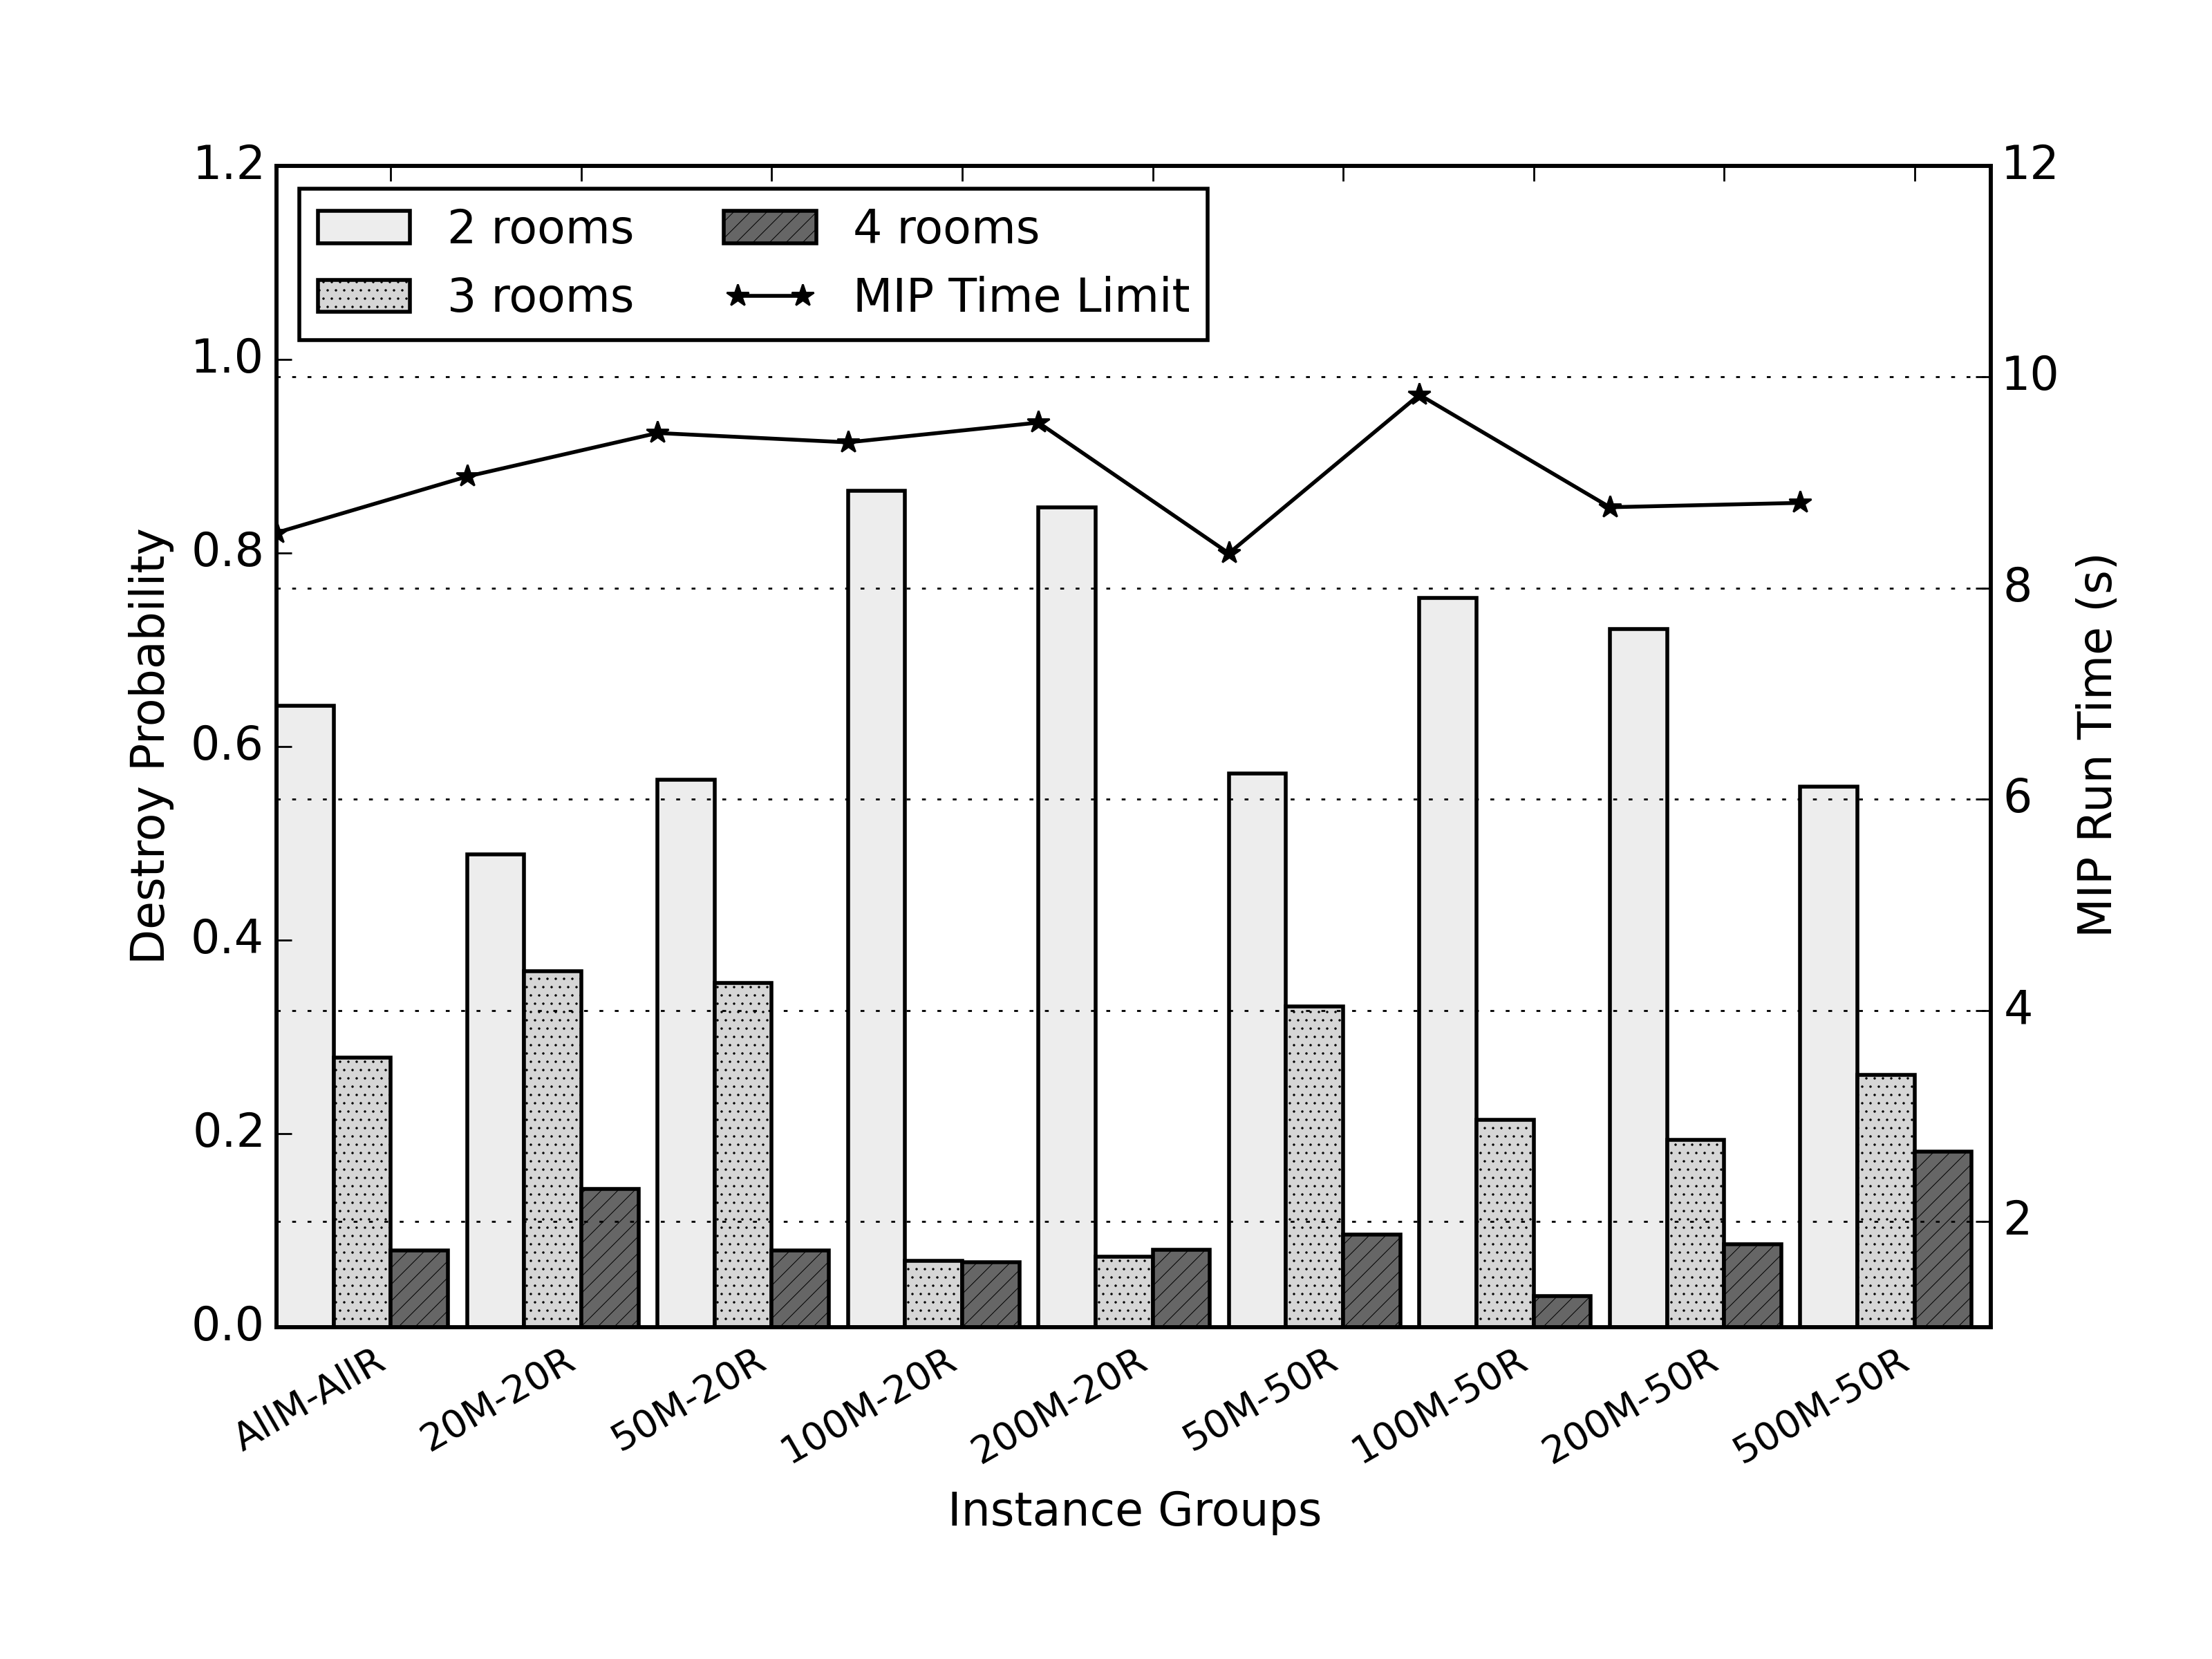
\includegraphics[width=0.9\linewidth]{figs/mipdestroy_1027.png}
	\caption{Parameter configurations as determined by SMAC.}
	\vspace*{-2ex}
	\label{fig:mipdestroy_0907}
\end{figure}

\begin{figure}
\centering	
	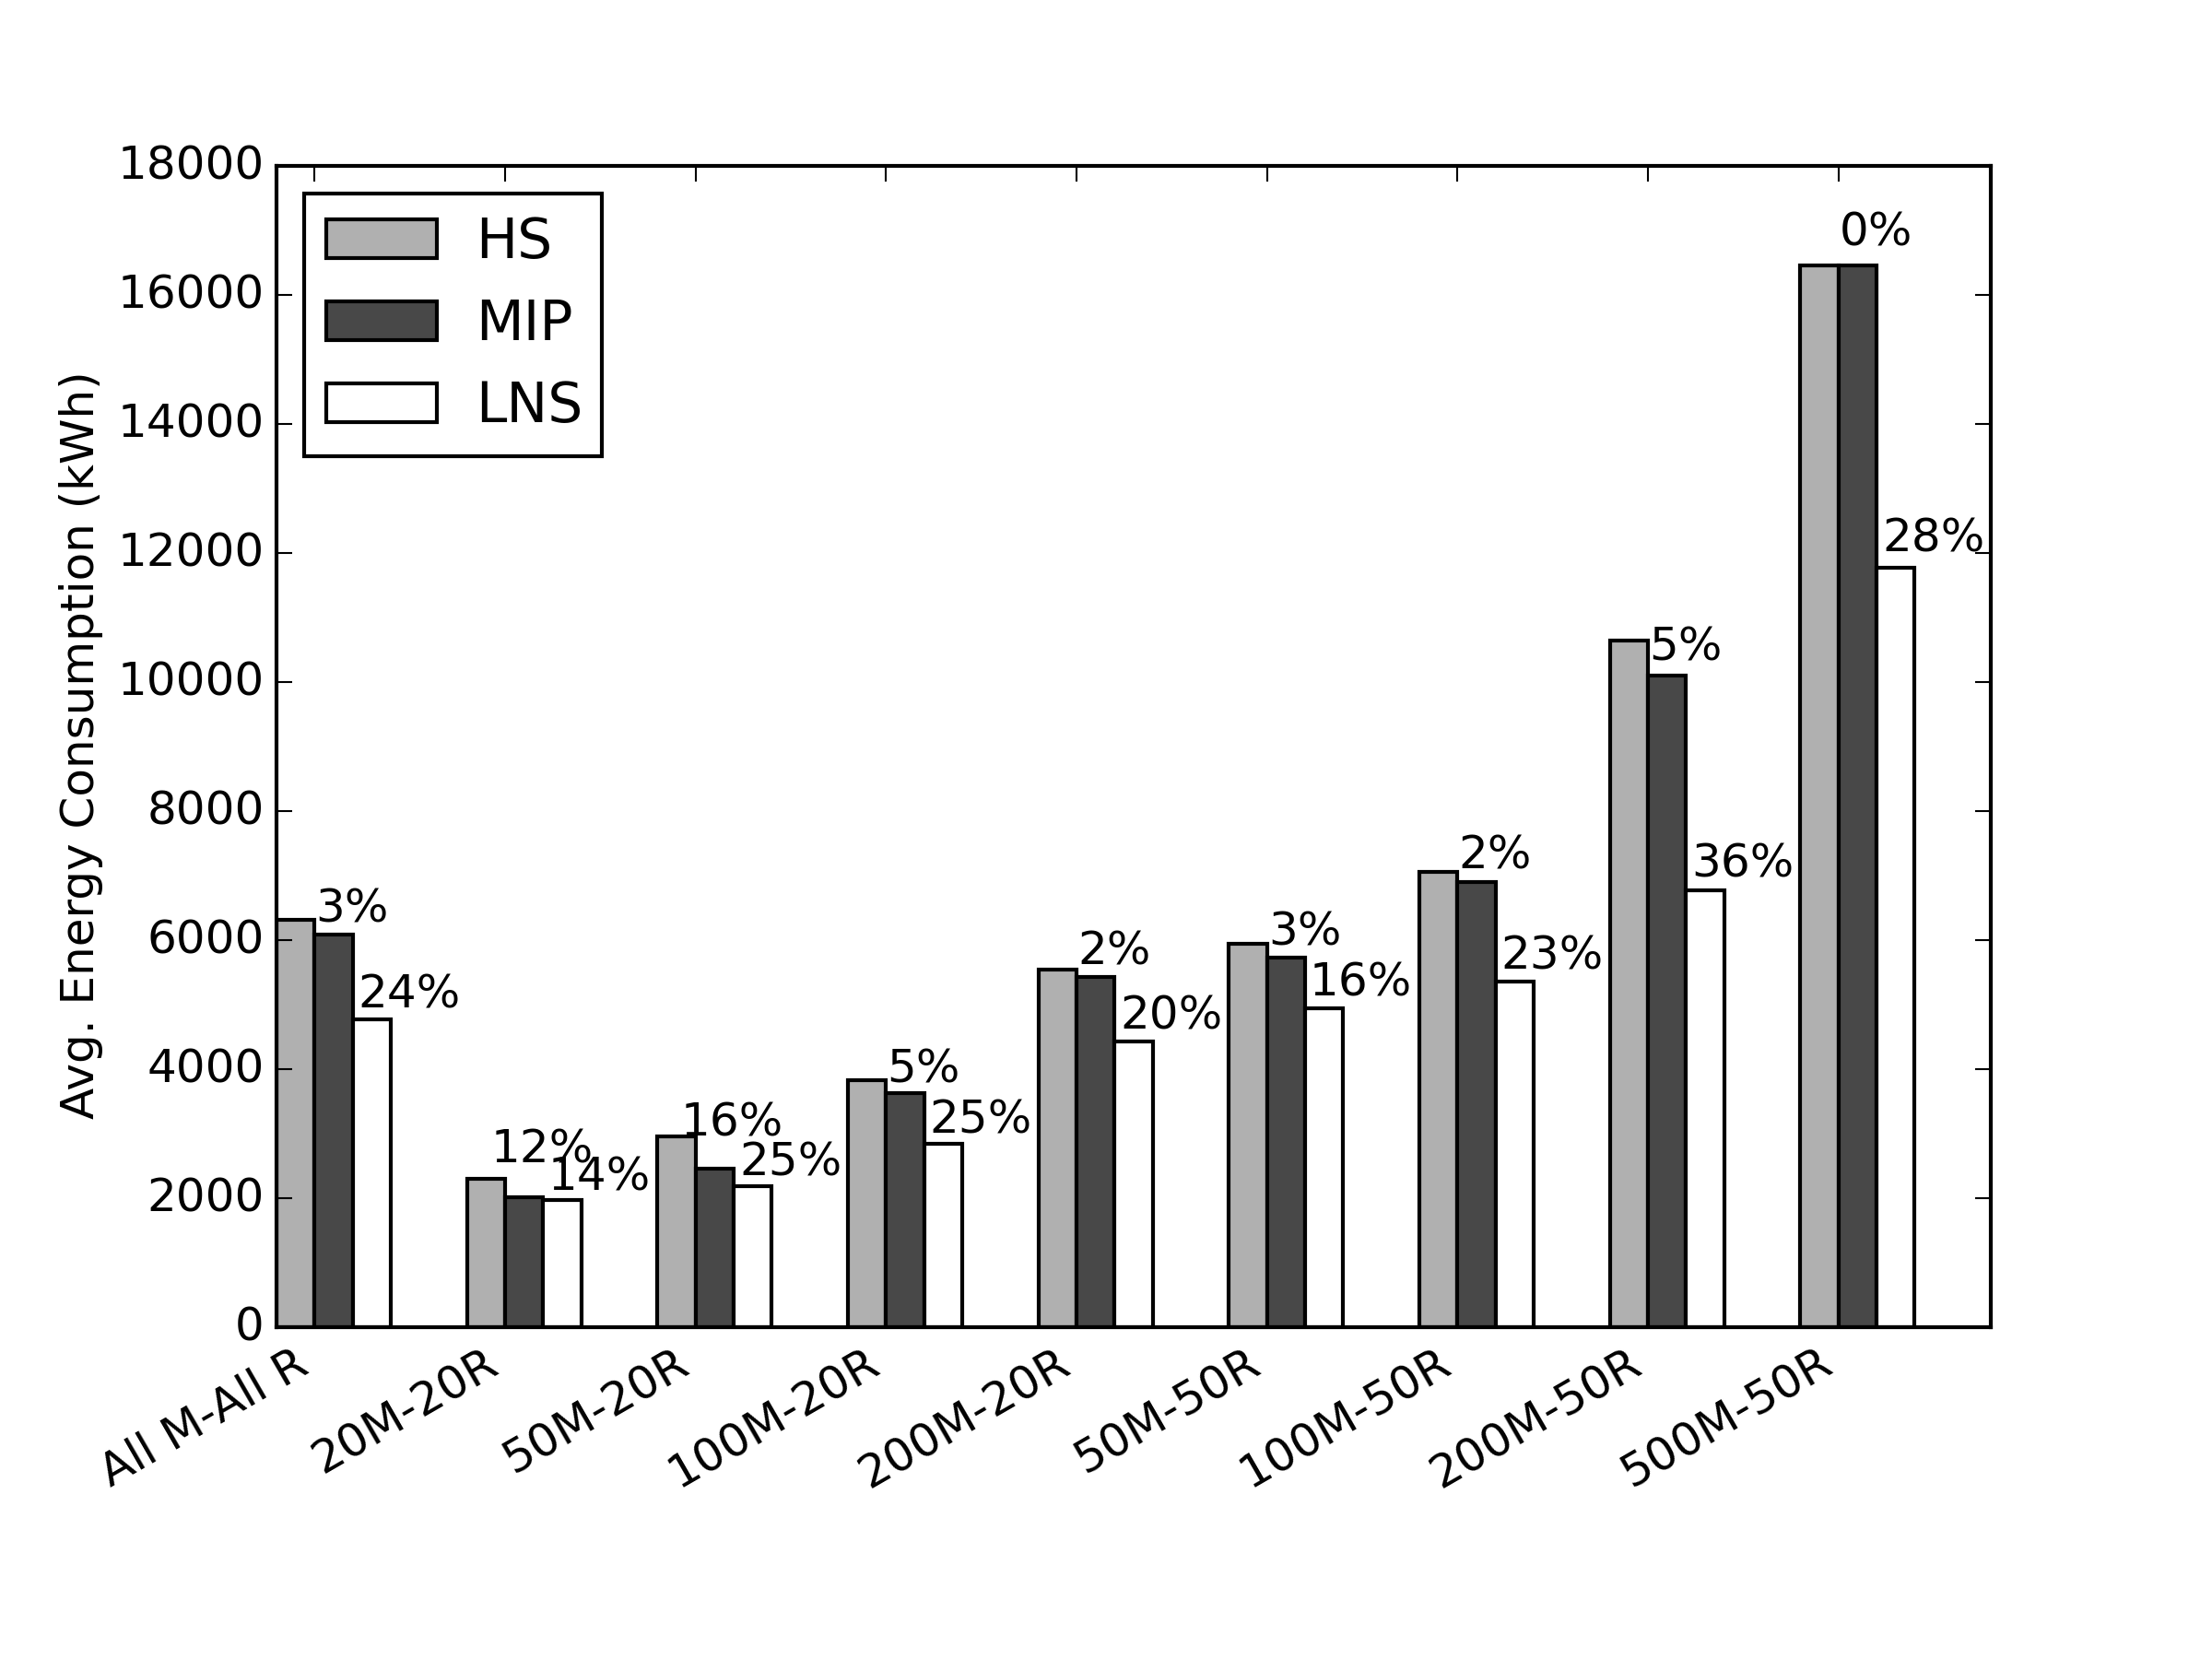
\includegraphics[width=0.9\linewidth]{figs/lnsmip_mspec_mspec900_shortHS_maxdata500.png}
	\caption{Performance improvement of MIP and LNS over heuristic solution (HS). MIP and LNS runtime 15 minutes.}
	\vspace*{-2ex}
\label{fig:mspec_mspec_900}
\end{figure}

First, we used SMAC to tune the parameters for all 80 instances. %It is, however, possible that the parameters of the LNS may have an impact on the performance of LNS when solving a problem instance.
However, it is possible that one set of parameter configurations might not produce best results across all problem sets.
For example, \cite{malitsky2013tuning} observed that instance specific algorithm configuration finds good quality solutions for large sized instances in limited time. Hence, second we independently tuned the parameters for the 8 problem sets. In each case, we used 0.33, 0.33, and 0.34 as the default destroy probabilities and 5 seconds for the default MIP runtime during each repair step. SMAC trains on 60\% of the instances and cross-validates with the remaining 40\%.

On average, SMAC generated 300 configurations for each problem set. Figure \ref{fig:mipdestroy_0907} shows the best parameter configurations as determined by SMAC for all 80 instances (AllM-AllR), and for the each of the 8 problem sets. In the end, a MIP runtime of 8.5 seconds, and probabilities of 0.64, 0.28, 0.08 to destroy 2, 3, and 4 rooms respectively were determined to be the best settings by SMAC for all 80 instances. However, the best parameter configurations do vary somewhat for the different problem sets.

\begin{figure}
	\centering
		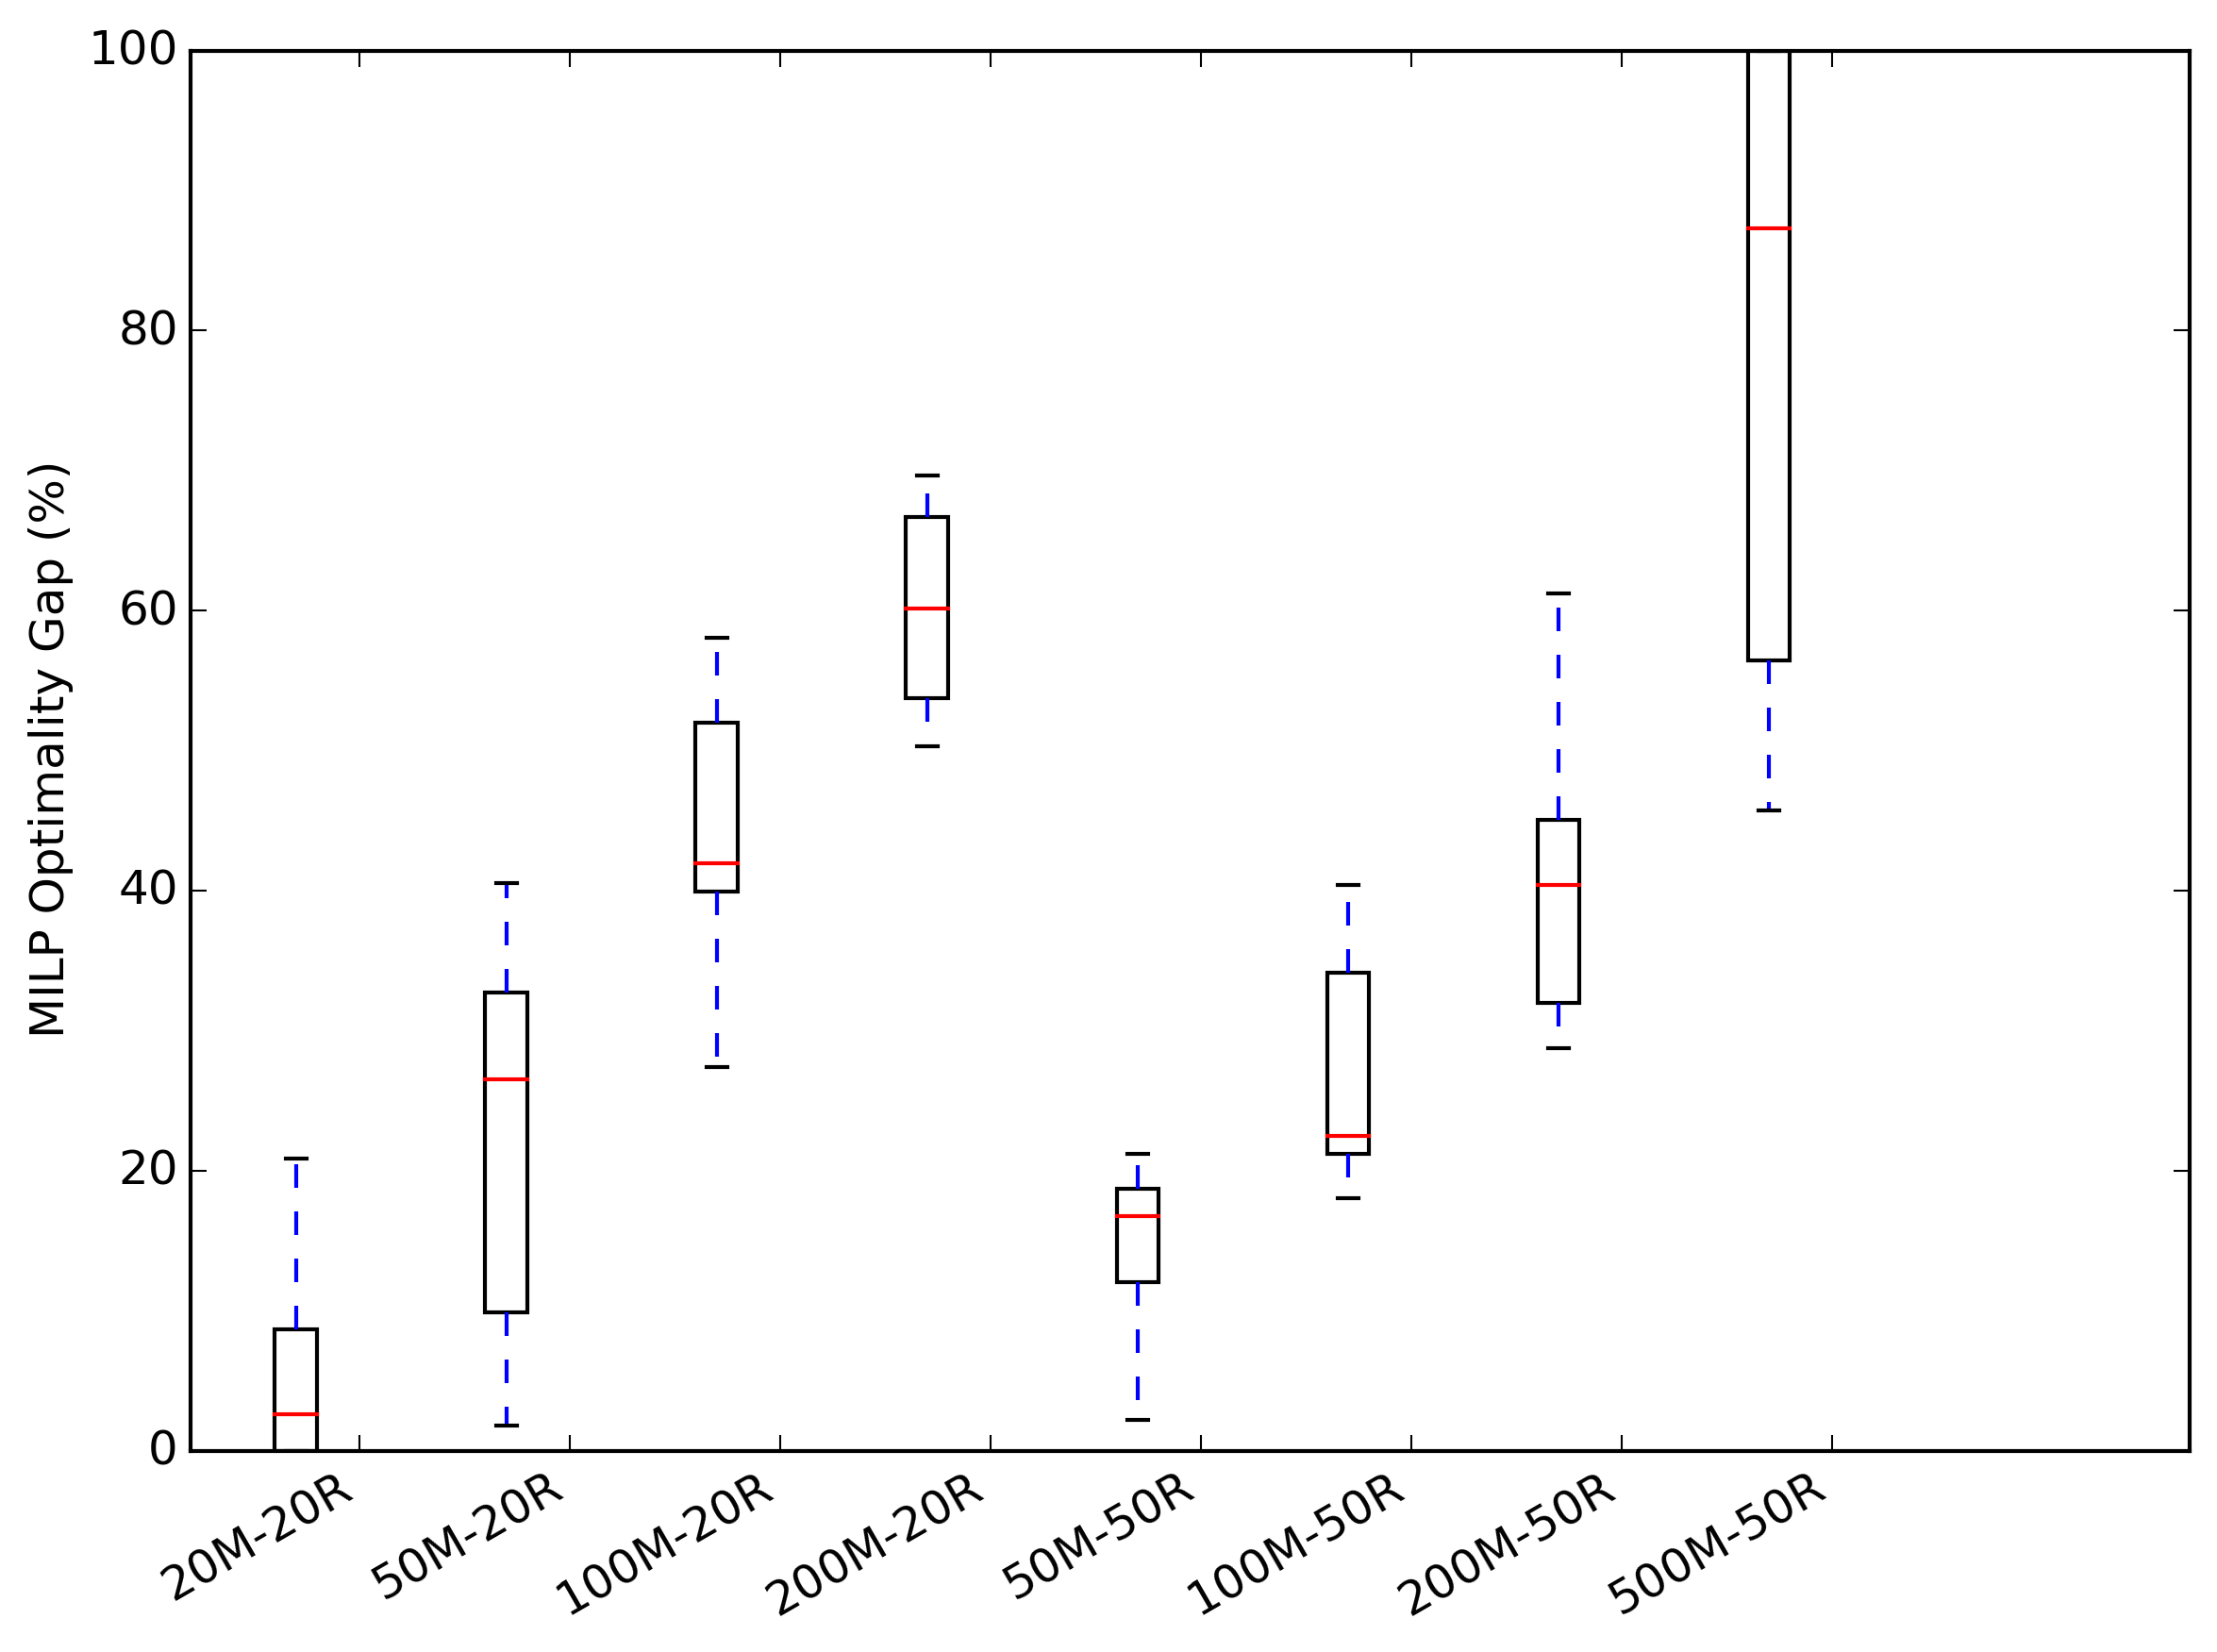
\includegraphics[width=0.9\linewidth]{figs/mip_optgap_maxdata500.png} \\
(a) MIP optimality gap \\[6pt]
		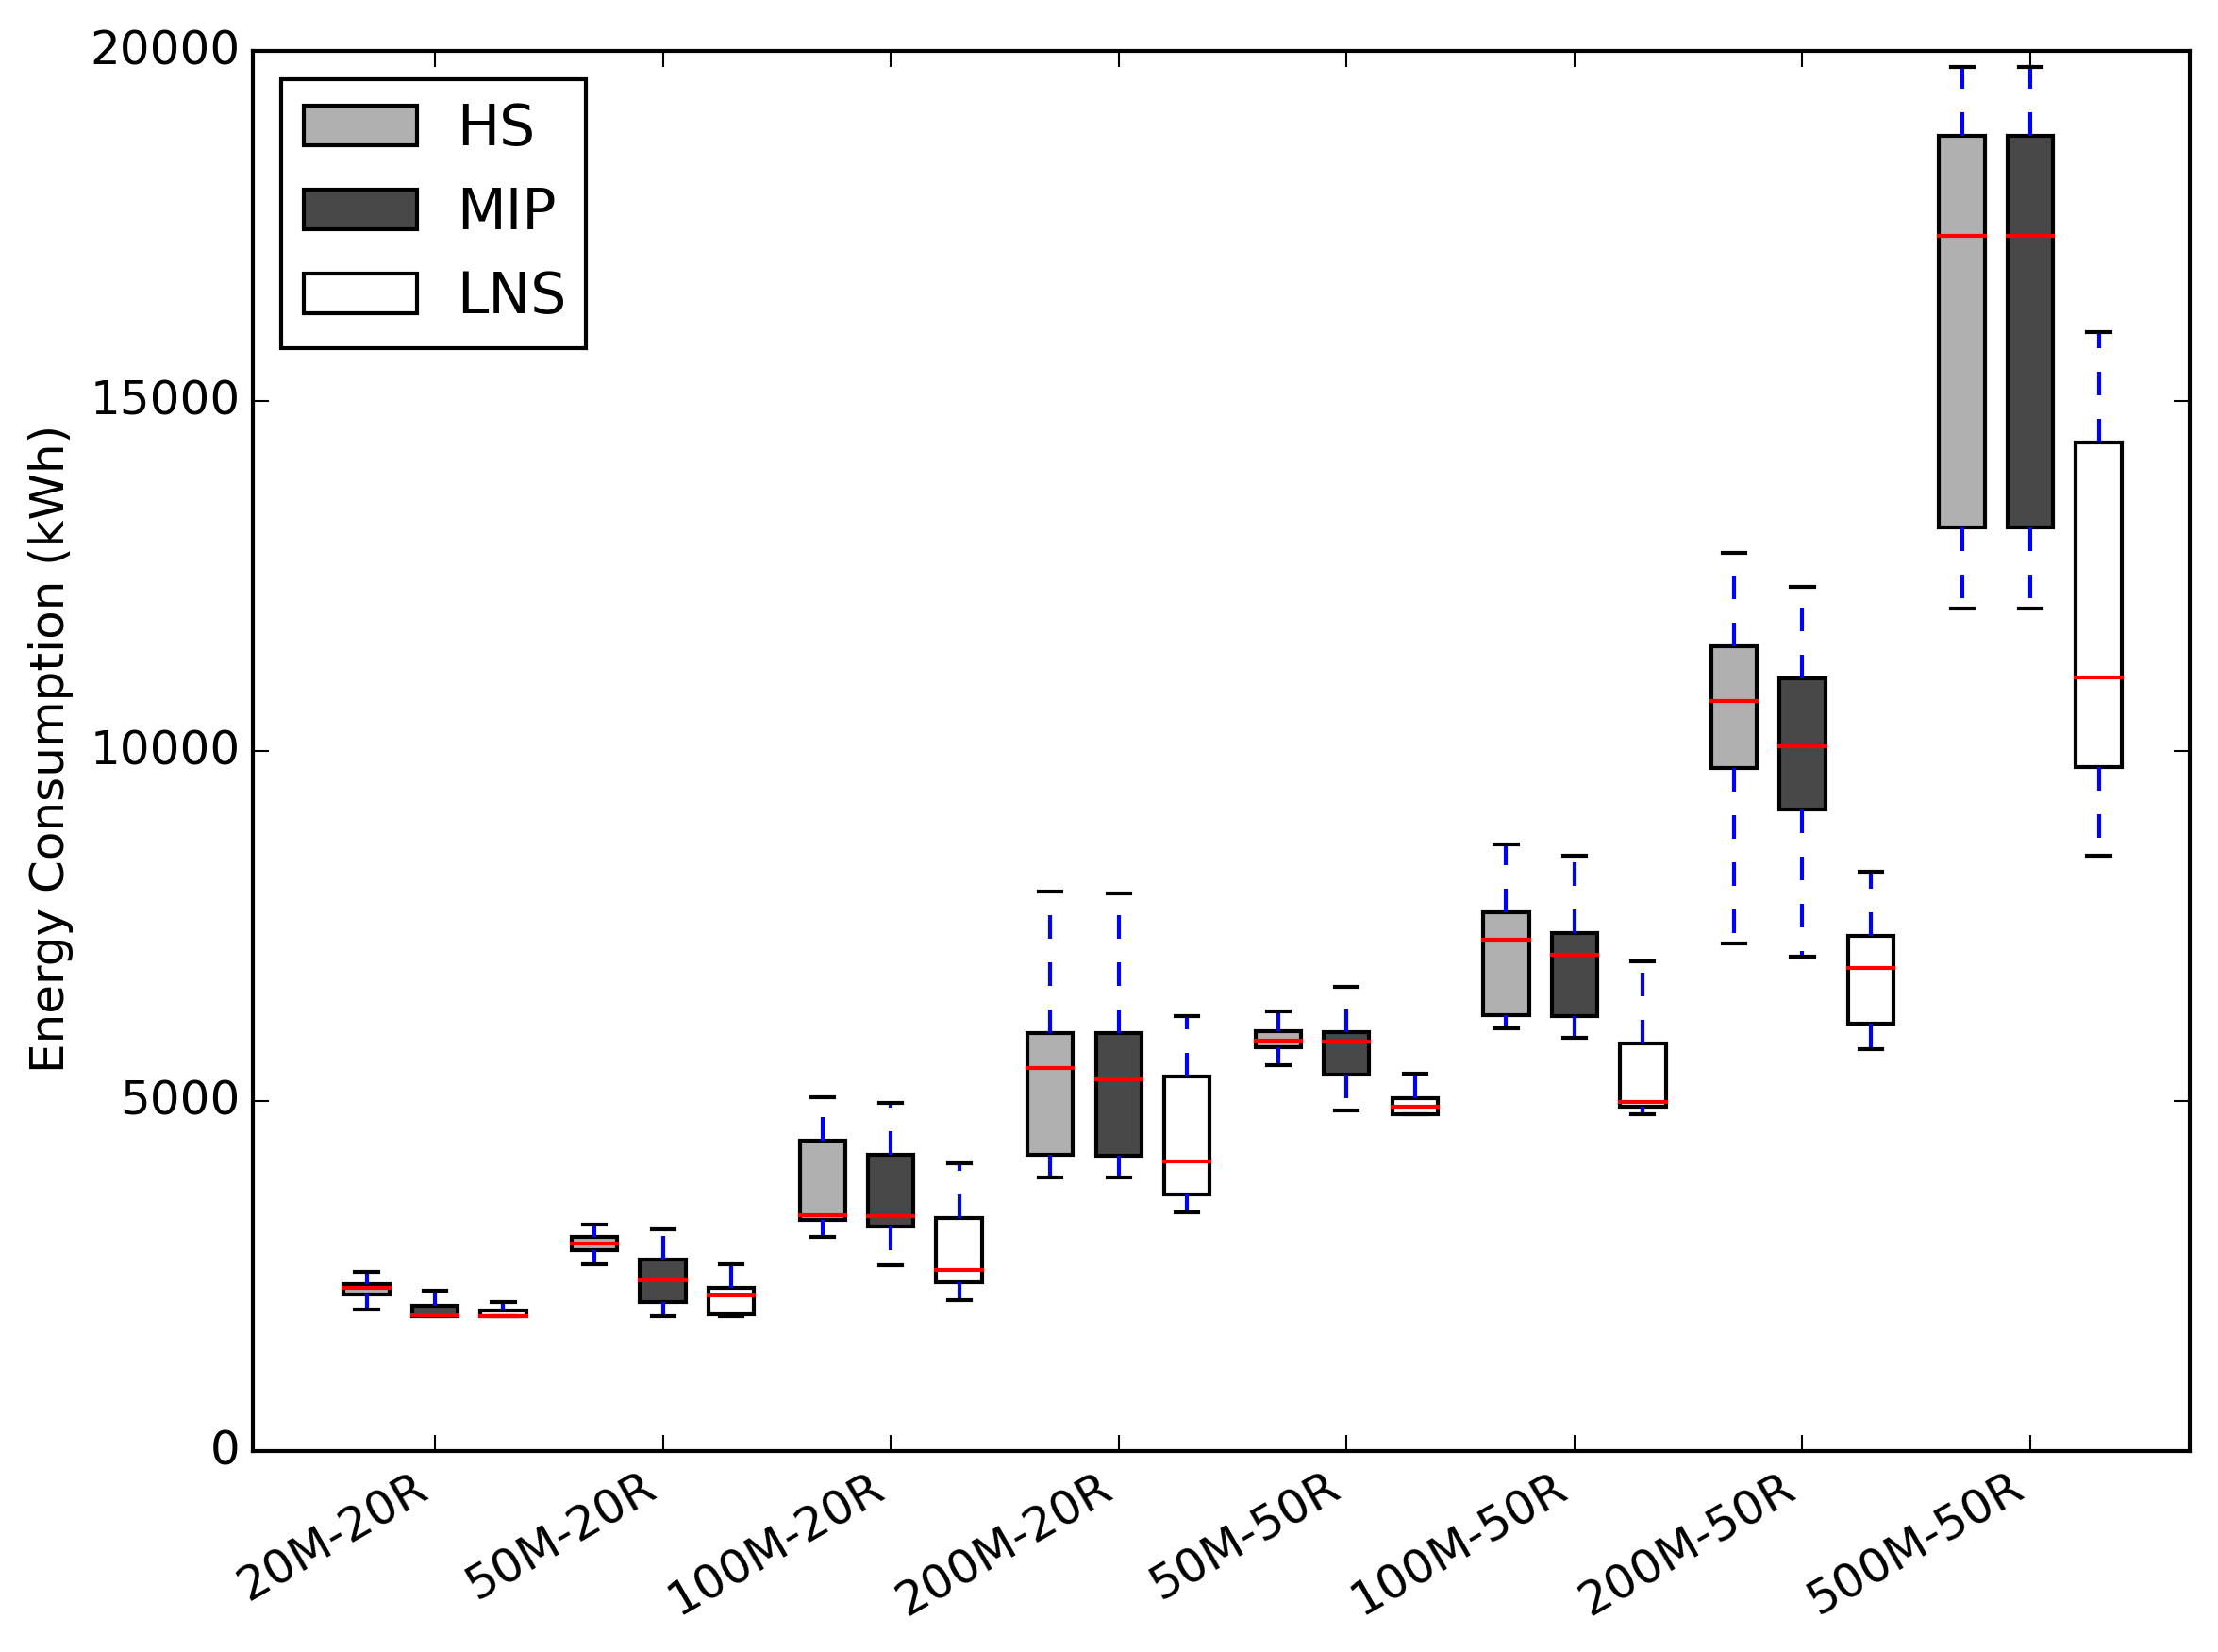
\includegraphics[width=0.9\linewidth]{figs/lnsmip_mspec_mspec900_shortHS_box_maxdata500.png}\\
(b) HS/LNS/MIP solution values \\[6pt]
	\caption{MIP optimality gap (top) and HS/LNS/MIP solution values (botton)}
	\label{fig:optgap}
\end{figure}

Figure \ref{fig:mspec_mspec_900} shows the performance improvement of MIP and LNS compared to the initial feasible solution, which is referred to as the heuristic solution (HS), over 500 runs. For each run, both the MIP and LNS approach were seeded with HS as an initial solution. Both MIP and LNS were given the same runtime limit of 15 minutes and HS was given 60 seconds. LNS was executed using the parameter configurations that were determined to be the best for each problem set. The results show that LNS significantly improves over MIP when given limited runtime. Overall, the improvement of LNS over MIP is between 14\% and 36\%. Note that in the largest problem instances, those in 500M-50R, MIP often fails to find even a slight improvement over the given initial solution HS in 15 minutes.

We reran all problem instances in Figure \ref{fig:mspec_mspec_900} using the AllM-AllR parameter settings. In this case, the performance of LNS decreased by 1 to 2\% for each problem set. Hence, instance specific algorithm configuration did have some impact, but even without it LNS performed significantly better than MIP.

Figure \ref{fig:optgap} provides insight into the optimality gap of the MIP approach and in the variation in solution quality. The MIP optimality gap after 15 minutes runtime is shown Figure \ref{fig:optgap}(a). Each box shows the median and the upper and lower quantiles of the optimality gap. The endpoints indicate the maximum and minimum. As observed previously the MIP approach fails to converge on the larger problem instances. Moreover, as can be seen from the figure, MIP's performance substantially degrades as problems become more constrained and exhibit a higher number of meetings to number of rooms ratio.

The variation in solution quality is shown on Figure \ref{fig:optgap}(b). The median of LNS always falls below the lower quantile of MIP. We note, however, that for the smallest problem instances in 20M-20R, MIP and LNS have almost similar performance. For even smaller problem instances MIP tends to be very effective, which is exactly why we have combined the two. We believe that the combination of LNS and MIP is especially good when considering highly constrained problems. LNS is used to destroy and repair the solution space and MIP is used to find a good local solution, possibly a locally optimal solution, in a short amount of time.



%\begin{figure}[h]
%\centering
%\begin{tabular}{cc}
%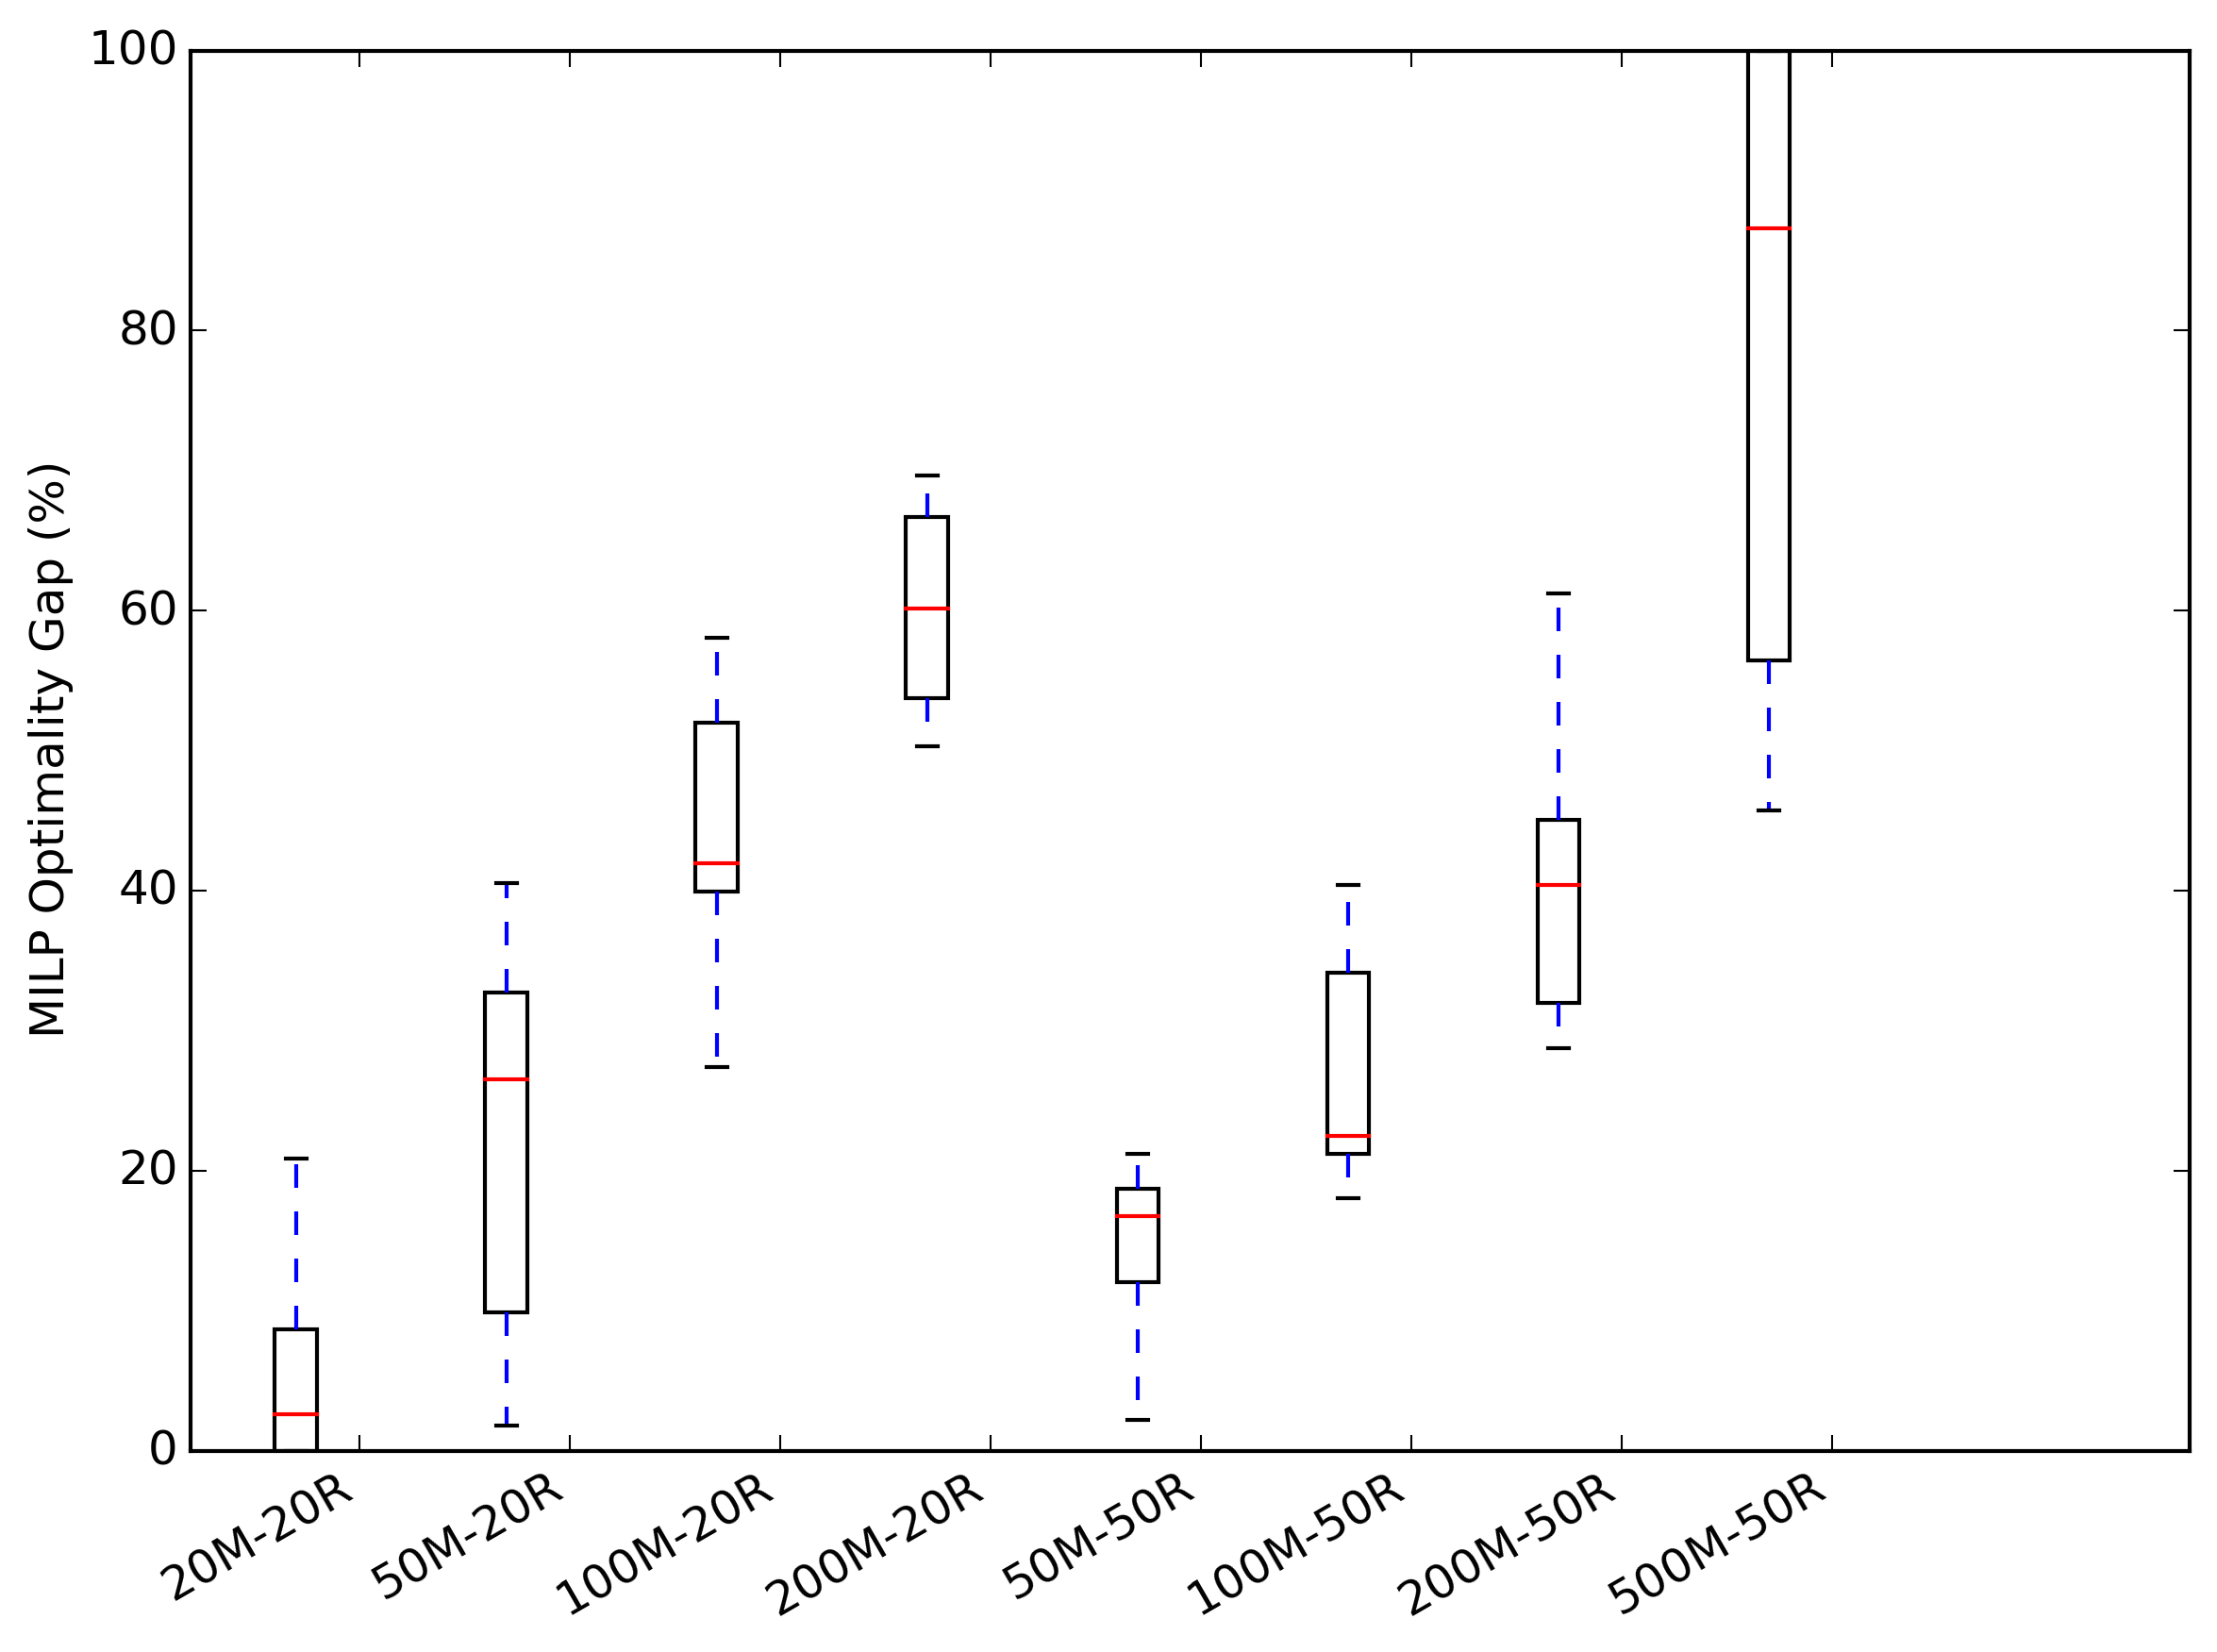
\includegraphics[width=2.3in,keepaspectratio]{figs/mip_optgap_maxdata500.png} &
%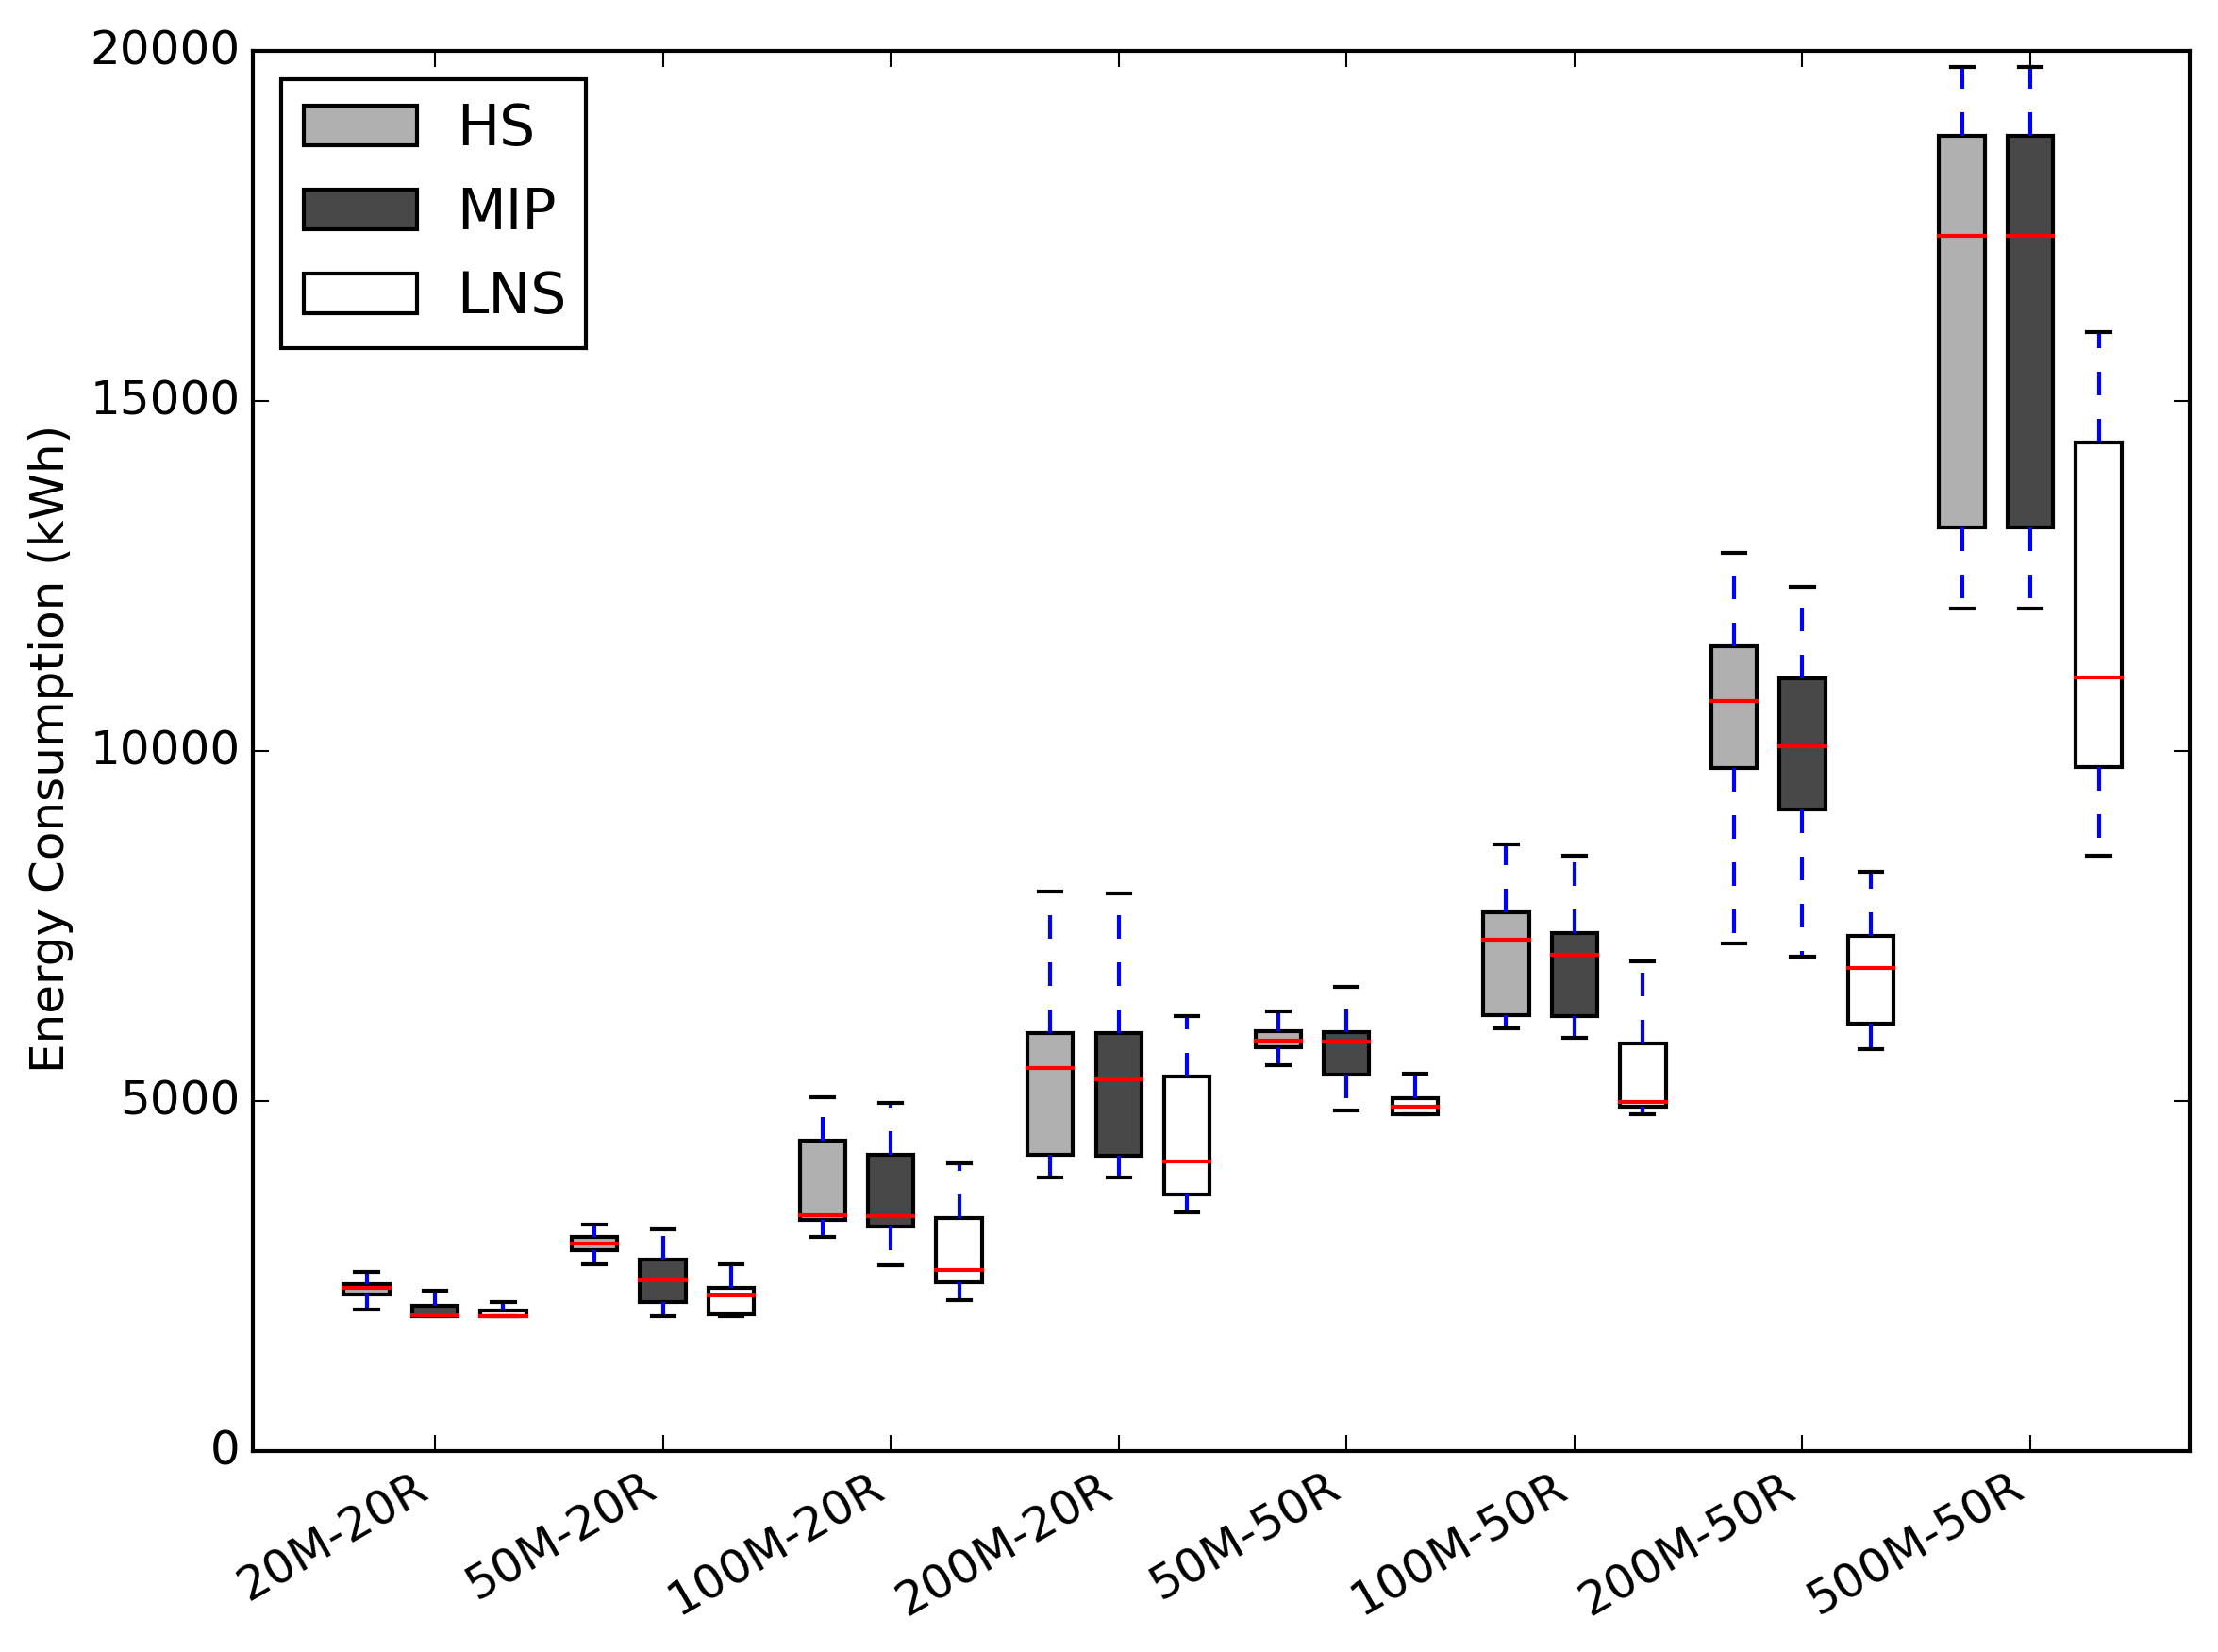
\includegraphics[width=2.3in,keepaspectratio]{figs/lnsmip_mspec_mspec900_shortHS_box_maxdata500.png} \\
%\end{tabular}
%\caption{MIP optimality gap (left) and HS/LNS/MIP solution values (right)}
%\label{fig:optgap}
%\end{figure}


\section{Related Work}\label{sec:related_work}

In Chapter \ref{cha:milp} we combine MPC with meeting scheduling and propose a MIP-based solution. This model achieves significant energy reduction when compared to approaches similar to those presented in \cite{goyal2013occupancy,kwak2013tesla,majumdar2012energy}. The drawback of this approach is that it does not scale well, which is why we developed a hybrid solution that combines MIP with LNS \citep{lim2015large}. %In \cite{lim15hvac}, we presented some of the initial results on applying LNS on this problem.  Here, we significantly expand on the details of the LNS algorithm, and present extensive results supporting the quality of the algorithm.

Also limited by the scalability of MIP, existing work on energy-aware scheduling only consider a small number of meetings or rooms. For example, \cite{chai2014minimizing} consider only 30 meetings in 9 rooms. \cite{kwak2013tesla} solves a total of 300 meetings per day in 35 rooms, but in an online manner where the MIP model needs to be solved at every session is relatively smaller. The other work resorts to heuristics-based approaches that generate a feasible solution in a reasonably short period of time but do not guarantee optimality. For instance, \cite{pan2013minimizing} examine up to 800 meetings in 150 rooms with their greedy scheduling algorithm. Likewise, \cite{majumdar2016characterising} only consider up to 12 meetings in 4 rooms due to the computational overhead incurred by feeding their schedules into building energy simulation software Energy+ \citep{crawley2000energyplus} for the calculation of HVAC consumption. Our work overcomes the limitations of these approaches by combining MIP with LNS, and by solving each sub-problem to optimality or near-optimality using a MIP-based integrated HVAC control and occupancy scheduling model. %scale well even for large instances.

There are techniques such as local branching or relaxation induced neigbourhood search (RINS) \citep{danna2005exploring,danna2003structured}, which apply local search to MIP. RINS forms a \textsl{domain-independent} neighbourhood in MIP. At every $n$th node of the MIP global branch-and-bound process, a MIP model is formed by fixing the value of the variables that have the same value in the current incumbent and the current continuous relaxation, and by solving on the remaining variables. The node limit $n$ is imposed to truncate the MIP optimisation when $n$ nodes have been explored in the search tree. 
% https://www.ibm.com/support/knowledgecenter/SS9UKU_12.5.0/com.ibm.cplex.zos.help/UsrMan/topics/discr_optim/mip/heuristics/45_rins.html
% Relaxation induced neighbourhood search (RINS) is a heuristic that explores a neighbourhood of the current incumbent solution to try to find a new, improved incumbent. It formulates the neighbourhood exploration as another MIP (known as the subMIP), and truncates the subMIP optimisation by limiting the number of nodes explored in the search tree.
In constrast, our model leverages a \textsl{domain-dependent} knowledge that forms a neighbourhood search strategy based on building zones and solves the joint HVAC control and occupancy scheduling sub-problem to optimality. The strength of our LNS model is that it allows a large neighbourhood to be explored using domain-dependent information whereas local branching or RINS explores a neighbourhood of the incumbent without using domain-dependent information. Moreover, RINS focuses on finding a good feasible solution instead of proving optimality. 
%   Note, we have not tried local branching on this problem, so this is something to test in future work.
% \cite{danna2003structured} --> In the literature, choosing related variables is most often achieved b taking advantage of the known high level structure of the specific problem at hand. Relaxation induced Neighborhood Search RINS) was introduced: it is a form of LNS that only relies on the continuous relaxation of the MIP model of the problem to define its neighbourhood. It can be used on any MIP model without any other input than the model itself. We want to investigate how a generic approach like RINS compares to a domain-dependent approach.
% combine structure and unstructured LNS (destroy room + RINS) - Use the LP relaxation to choose a neighbourhood Relaxation Induced Neighborhood Search (RINS) [Danna, Rothberg, Le Pape, 2003]

Parameter tuning is one important aspect of LNS. The values of the parameters of a LNS algorithm can impact the solution quality. These include the size of the neighbourhood, thresholds in terms of run time limit, node limit or solution limit etc. These parameters can be tuned based on knowledge of experts, or using an automated procedure. While we have only four configurable parameters in our LNS algorithm, it is impractical to examine all configurations. We resort to automated parameter tuning that adopt machine learning techniques.  Various parameter tuning software exist to automate the tuning process \citep{thornton2013auto,bergstra2012random, hutter2011sequential}. We use SMAC \citep{hutter2011sequential} to train our LNS parameters automatically and identify a global configuration that are optimum to tackle multiple instances of different features and properties. 
Note that SMAC has been used to train parameters in various applications such as kidney exchange matching \citep{dickerson2015futurematch}, medical imaging \citep{angermueller2016deep} and social network analysis \citep{vaswani2016adaptive} etc., but is first used here to train parameters in energy aware scheduling in smart buildings.

Combining constraint-based methods with neighbourhood search methods is not new. For example, \cite{lebras2013robust} use LNS with MIP in network design for a species conservation problem, \cite{gaspero2013constraint} use LNS with CP in balancing bike sharing systems, \cite{rendl2012hybrid} apply CP with variable neighbourhood search for home-care scheduling, \cite{mehta2012comparing} use both MIP and CP-based LNS approach for machine reassignment problem, \cite{bent2004two}, \cite{kilby2011flexible} use LNS with CP to solve vehicle routing problem, \cite{mitrovicminic09local} apply variable neighborhood search to the multi-resource generalized assignment problem. LNS is also widely used as a technique to solve complex timetabling problems \citep{meyers2006very,abdullah2007investigating,burke2010hybrid}, nurse rostering problems \citep{bilgin2012local} and shift-scheduling problems \citep{quimper2010large}. We are, however, unaware of its application in the space of energy aware scheduling in smart buildings.



\section{Conclusion and Future Work}\label{sec:lns:conclusion}

In this chapter we extend our work in Chapter \ref{cha:milp} which introduced a MIP model for energy aware meeting scheduling. The MIP model that is described previously only solves problem instances that involve a small number of meetings and rooms. We combine MIP with LNS % in order to scale to larger problems. 
and show that by embedding MIP model into a large neighbourhood search, we can scale to timetabling problems of practical relevance.

We developed a heuristic to generate an initial feasible solution quickly, which we use to warm start both the MIP and LNS approach. In our experiments, the most effective neighbourhood was one that destroys and repairs all meetings scheduled in 2 to 4 rooms. The resulting subproblem was small enough for MIP to solve to (near) optimality and, at the same time, large enough to explore alternate solutions. We studied the performance of MIP and LNS and demonstrated the potential of our LNS approach for effectively tackling large-scale HVAC control and meeting scheduling problems. The LNS achieves 14 to 36\% better energy savings than the MIP approach when both given a runtime of 15 minutes. 
%In order to provide an absolute sense of the solution quality, we plan to evaluate our schedules with the EnergyPlus simulator.

In future, we are interested in exploring new algorithmic approaches that allows us to scale even further. We are particularly interested in investigating symmetry breaking in MIP \citep{ostrowski2015modified}. Symmetries lead to a large number of equivalent solutions, which causes branch-and-bound to be ineffective. While we dealt with symmetries due to meetings with similar characteristics by introducing meeting types, symmetries still exists in our MIP formulation due to rooms with similar characteristics. Introducing room types, however, may not be possible because room temperature at time step $t$ is dependent on time step $t-1$. In future work, we aim to identify branching strategies that can better deal with symmetries in our MIP formulation, for example, by assigning different branching priority to variables $x_{m,l,k}$ such that rooms with different energy consumption are explored first. %On top of that, most of the existing optimisation solvers \citep{gurobi, cplex2009v12} provide a configurable symmetry breaking parameter that, once activated, automatically detect and remove symmetries. It might be interesting to activate this parameter while running the repair step.

We will also further investigate incorporating RINS-based local branching to our LNS model. This can be achieved by activating RINS  heuristics in MIP solvers such as \cite{gurobi}. It will be interesting to compare the solution quality of these approaches.
For the initialization stage of LNS, it might also be possible to formulate the initial schedule using different heuristics, modeling and solving technique such as CP. 



%Moreover, we are also interested in investigating an online stochastic approach to our HVAC control and meeting scheduling problem. Such an approach can deal with current requests, future requests, changes and cancelation of requests, but also with the uncertainty around outdoor air temperature and weather conditions.

%This approach may also be further enhanced to incorporate dynamic temperature bounds to adjust thermal comfort based on outdoor temperature. %It is expected to greatly reduce the energy consumption while improving the solution feasibility.

